\chapter{Introduction}\label{chp:chp1}

\begin{flushright}
  {\em ``The mind loves the unknown. It loves images whose meaning is unknown, since the meaning of the mind itself is unknown.''}\\

\ \

\normalsize
{Ren\'e Magritte}
\end{flushright}


\noindent{In this introductory chapter, I present the main topics necessary to understand the contents and motivation of this thesis. I start from an introduction to cosmology in Section \ref{sec:cosmology}. Sections \ref{sec:clusters} and \ref{sec:introgw} introduce the main areas treated in my work, galaxy clusters and gravitational waves, with focus on topics which are relevant within the Dark Energy Survey (DES). DES and other galaxy surveys are described in Section \ref{sec:surveys}.} %In particular, I stress the importance of galaxy evolution studies for clusters cosmology and gravitational wave optical follow ups.}

\section{Cosmology}\label{sec:cosmology}

The most accepted cosmological model nowadays is called the Friedmann-Robertson-Walker (FRW) Model, also known as the Standard Cosmological Model (SCM). In this model the geometry of the Universe is described by the Robertson-Walker (RW) metric, that can be derived assuming the Cosmological Principle, which says that ``the Universe is homogeneous and isotropic on large scales''. This principle is observationally verified over the fraction of Universe that we can see, the \emph{Observable Universe},  that corresponds more or less to the present \emph{Hubble Volume} (a few $\textrm{Gpc}^3$). The transition towards homogeneity is indeed clear from the galaxy surveys on scales greater than a megaparsec, and in the Cosmic Microwave Background (CMB) anisotropies (which are roughly only one part over $10^5$).
Although the observational evidence does not imply either that the entire Universe has these features, or that the region of the Universe we live in will last in this state forever, we can affirm that it will conserve these properties at least for the time needed to cross it at the light velocity, the \emph{Hubble time}, estimated around $10$ Gyr. So, in order to understand the Observable Universe, we first begin by describing its overall background evolution as if it were isotropic and homogeneous, neglecting the inhomogeneities that we observe today on small scales.\\

Unless otherwise stated, quantities are expressed in units such that for the light velocity $c=1$ in this Section. Further information about the Standard Cosmological Model might be found in Dodelson's monograph (\citealt{dodelson}) or in \citet{kolb}.

%%%%%%%%%%%%%%%%%%%%%%%%%%aggiungi f_k
%----------------METRICA RW------------------------------------%
\subsection{Robertson-Walker Metric}
The isotropy and homogeneity assumptions imply that all the spatial coordinates evolve in time in the same way, and that in a metric $g_{\mu\nu}$ terms like $g_{0 j}$ ($j= 1, 2, 3$) are zero. It can be then proven that the RW metric can be written in a general way as:
\begin{equation}
ds^{2} = dt^{2} + h_{ij}dx^{i}dx^{j} = dt^{2} - a^{2}(t)dl^{2}, \label{RW}
\end{equation}where $a(t)$ is the \emph{scale factor} that describes the Universe dynamics on large scales, $t$ is the proper time measured by an observer standing in the comoving reference frame (that means, in polar coordinates, $r,\theta,\phi = constants$), $h_{ij}$ is the metric tensor restricted to spatial coordinates (such that if $g_{\mu \nu}$ is the metric tensor, $h_{ij} = - g_{ij}$, $i, j= 1, 2, 3$), $dl^{2}$ is the spatial line element of a three-dimensional space with constant positive, negative or zero curvature.
It can be proven that in spherical coordinates, $(r, \theta, \phi)$, the line element is described by:
\begin{equation}
ds^{2} = dt^{2} - a^{2}(t) \Big \{ \frac{dr^{2}}{1-kr^2} + r^{2}d\theta^{2} + r^{2}\sin^{2}{\theta} d\phi^{2} \Big\} , \label{RW4}
\end{equation}where $k = 0, 1, -1$ for respectively zero, positive or negative curvature.%\footnote{With non-zero curvatures, it is always possible to redefine $r$ and $a$ in a way such that $k=\pm 1$.}

%Before studying the kinematics of a particle in a RW space, we write down the non-zero components of the Christoffel symbols:
%\begin{eqnarray}
%\Gamma^{i}_{jk} & = & \frac{1}{2} h^{il} \Big( \frac{\partial h_{lj}}
%{\partial x^{k}} + \frac{\partial h_{lk}}{\partial x^{j}} - \frac{\partial h_{jk}}{\partial x^{l}} \Big)\,, \\
%\Gamma^{0}_{ij} & = & \frac{\dot{a}}{a} h_{ij} \label{RW7}\,,\\
%\Gamma^{i}_{0j} & = & \frac{\dot{a}}{a} \delta^{i}_{j} \,, \label{RW8}
%\end{eqnarray}of the Ricci tensor:
%\begin{eqnarray}
%R_{00} & = & -3 \frac{\ddot{a}}{a}\,,\\
%R_{ij} & = & -\Big( \frac{\ddot{a}}{a} + 2 \frac{\dot{a}^{2}}{a^{2}} + \frac{2k}{a^{2}} \Big) g_{ij}\,, \label{RW6}
%\end{eqnarray}and the Ricci scalar:
%\begin{equation}
%\mathcal{R} = -6 \Big( \frac{\ddot{a}}{a} + \frac{\dot{a}^{2}}{a^{2}} + \frac{k}{a^{2}} \Big)\,. \label{RW9} 
%\end{equation}

\subsection{Redshift and Astrophysical distances}
The motion of a free test-particle is described by the geodesic equation, which can be simplified in the RW metric to:
\begin{equation}
\frac{\dot{u}}{u} = -\frac{\dot{a}}{a}\, , \label{RW11}
\end{equation}
where $u$ is the spatial velocity of the particle. This differential equation admits the solution $u \propto a^{-1}$, which has a fundamental consequence: if $m_0$ is the rest mass of the particle, its momentum $p=m_0u$ scales as $a^{-1}$, 
therefore it changes if the Universe expands or contracts. We can therefore apply this same reasoning for a particle following $ds=0$, that is a particle with zero mass. So, for a photon of energy $\varepsilon$, if its wavelength is $\lambda$:
\begin{equation}
\varepsilon = p = \frac{2\pi}{\lambda} \propto a^{-1}.
\end{equation}Hence if a photon is emitted from a source at time $t_{em}$ with wavelength $\lambda_{em}$, it will be observed at time $t_{oss}$ with a greater wavelength $\lambda_{oss}$ if the Universe is expanding (\emph{redshift}), or with a smaller wavelength if it is contracting  (\emph{blueshift}); in fact:
\begin{equation}
1+z \equiv \frac{\lambda_{oss}}{\lambda_{em}} = \frac{a(t_{oss})}{a(t_{em})},\label{eq:z}
\end{equation}where the redshift $z$ was introduced.
In the same way, any proper length $l$ varies with the expansion or contraction of the space, and as a consequence the only physical, measurable length becomes $a(t)l$. This fact led astrophysicists to a redefinition of distances. 

The fundamental distance measure, the one from which all other distances can be computed, is that in the comoving reference frame. An important comoving distance is that between a distant photon emitter and us:\footnote{$t_0$ refers to the present time.}
\begin{equation}
\chi(a)=\int_{t(a)}^{t_0}\frac{dt'}{a(t')}\,.\label{comovingdistance}
\end{equation}

On the other hand, the \emph{proper distance}, the length of the spatial geodesic between two points, is:
\begin{equation}
d_p \equiv a(t)\chi,
\end{equation}where $\chi$ is the radial comoving distance. %It can be obtained by integrating the metric over the radial component (and neglecting the other coordinates which are zero along a geodesic\footnote{so it is finally the same of \reff{comovingdistance}.}).

Moreover, the  \emph{luminosity distance} $d_L$ is defined as:
\begin{equation}
d_L^2 \equiv \frac{\mathcal{L}}{4 \pi \mathcal{F}},
\end{equation}where $\mathcal{F}$ is the energy measured per unit time and area, and $\mathcal{L}$ is the luminosity (energy per unit time). Supposing that the emitted radiation propagates isotropically in space, from the definition it is clear that  $d_L$ would be the distance to the source if there were no expansion of the space. On the other hand, in case of expansion, light emitted from a position at $\chi$ in the comoving reference frame arrives at our position, which we choose to be at $\chi=0$, crossing an area of $4 \pi a_0^2 \chi^2=4 \pi \chi^2$.\footnote{It is usual to take $a_0=1$.} Moreover, its photons will lose a factor $(1+z)^2$ of their energy, of which $(1+z)$ comes from the greater distance travelled, and the other $(1+z)$ from the growing of the proper wavelength. Consequently from energy conservation:
\begin{equation}
\mathcal{F} = \frac{\mathcal{L}}{4 \pi \chi^2 (1+z)^2} \qquad \Longrightarrow \qquad d_L = \chi (1+z)=\frac{\chi}{a}\,. \label{RW14}
\end{equation}
A classic way to measure distances in astronomy is through the angle $\vartheta$ subtended by an object of physical length $l$. The \emph{angular diameter distance} is then defined as:
\begin{equation}
d_A\equiv \frac{l}{\vartheta} = d_L/(1+z)^2\,,
\end{equation}which we have also expressed in terms of the luminosity distance, and has an explicit expression that depends on the curvature of the Universe.


%---------------------Hubble law---------------%
\subsection{Hubble Law\label{hubblelaw}}
The Hubble Law describes, to a first approximation, the relative recession of galaxies, and it can be analytically derived by considering galaxies as travelling along geodesic in a RW metric. %\footnote{As RW metric assumes a maximal spatial symmetry, local irregularities must be neglected in order to obtain this law that holds true only over large scales. Concerning this, it is worth noting that: \begin{itemize}
%\item the galaxies recession does not consist of a proper physical motion, but rather of an increase of distances due to a geometrical expansion;
%\item gravitationally bound systems such as galaxies, clusters, superclusters, etc., once formed, follow the expansion only as a single system, and the metric in the inner parts might be considered as flat.
%\end{itemize}}
Expanding $a(t)$ in a Taylor series around the present time (which means obtaining the Hubble Law for a time around ours, or rather for Universe regions close enough to us):
\begin{equation}
\frac{a(t)}{a_0} \equiv \frac{1}{1+z} = 1 + H_0(t-t_0) - \frac{1}{2} q_0H_0^2(t-t_0)^2 + ...\,, \label{RW13}
\end{equation}where the subscript $0$ indicates the quantities evaluated at present time. Defining the \emph{Hubble Parameter} $H(t)=\dot{a(t)}/a(t)$, the Hubble Parameter at present time, called the \emph{Hubble constant}, is:
\begin{equation}
H_0 \equiv \frac{\dot{a_0}}{a_0},
\end{equation}and the \emph{deceleration parameter}
\begin{equation}
q_0\equiv -\frac{\ddot{a_0}}{\dot{a_0}^2} a_0 = -\frac{\ddot{a}}{a H_0^2}.
\end{equation}
Another useful definition is the \emph{Hubble length} $L_H \equiv H(t)^{-1}$, that approximatively represents the distance that a photon can travel\footnote{Note that units with $c=1$ are used.} in a Hubble time $H^{-1}$, and it is the scale that has to be compared to the characteristic length of any physical process in order to understand whether such a process might cause cosmologically relevant effects or not. One can similarly compare the characteristic time  $\tau$ of a reaction to $H^{-1}$, \emph{i.e.} a process needs to be faster than expansion in order to be able to maintain the equilibrium. Comparing $H$ with the reaction rate $\Gamma$ is often preferred.\\
At small distances, \reff{RW14} becomes the Hubble Law:\footnote{Interpreting the redshift $z$ a a Doppler effect, obtaining the Hubble Law in the classical form $v=H_0 d$ is straightforward.}
\begin{equation}
H_0 d_L = z + \frac {1}{2} (1-q_0)z^2 + ...\label{boh}
\end{equation}
It is worth stressing that the luminosity distance is not necessary in order to obtain the Hubble Law, but for the close distances that we are considering in this approximation, the proper distance $d = a(t)\chi$ works as well. Eq. (\ref{boh}) is however useful when \emph{Standard Candles} are observed, because $d_L$ is the observable in such case.

Note that the approximations used imply that for galaxies not satisfying $z \ll 1$, the relationship between $d_L$ and $z$ differs from the Hubble law, in a way that depends on the cosmological model: we need a solution $a(t)$ from Einstein's equations in order to obtain an exact expression of $r$. Einstein's equations are treated in the next section.

%AGGIUNGERE LE ALTRE DISTANZE! ORIZZONTE... e angolare?
%---------------------Universe dynamics----------------%
\subsection{Dynamics of the Universe}
In order to obtain an expression for $a(t)$, let us write the Einstein equations:
\begin{eqnarray}
R_{\mu \nu} - \frac{1}{2} \mathcal{R} g_{\mu \nu} & = & G_{\mu \nu} \\
& = & 8 \pi G T_{\mu \nu} + \Lambda g_{\mu \nu}, \label{einstein}
\end{eqnarray}where  $G_{\mu \nu}$  is the Einstein tensor, $T_{\mu \nu}$ is the stress-energy tensor, $\Lambda$ is the cosmological constant. 

For a perfect fluid in a space that satisfies the cosmological principle, $T_{\mu \nu}$ has a particular form, since homogeneity, isotropy and the absence of viscosity impose zero off-diagonal components and equal diagonal elements for the space components. If $\rho$ is the energy density of the fluid and $P$ its pressure:
\begin{equation}
T_{\mu \nu} = diag (\rho, -P, -P, -P). \label{tmunu}
\end{equation}

The Friedmann equation is the $\mu = \nu = 0$ equation of Einstein's equations, that in a RW metric becomes:
\begin{equation}
\frac{\dot{a}^{2}}{a^{2}} + \frac{k}{a^{2}} = \frac{8 \pi G}{3} \rho,\label{friedmann}
\end{equation}
while the acceleration equation can be written as:
\begin{equation}
\frac{\ddot{a}}{a}= -\frac{4 \pi G}{3}(\rho + 3P).\label{accelerazione}
\end{equation}
If today there is expansion ($\dot{a}\ge 0$), and if $\rho + 3P > 0$ has always held, as expected by the Standard Cosmological Model, this equation tells us that $\ddot{a}$ has always been negative, implying that there must have been a certain time in the past when $a=0$. That time, when the Universe was concentrated in a singularity, is often chosen as the ``zero-time''.\\
According to the SCM, the Universe has not always evolved in the same way. In fact, from the energy conservation ($T^{0 \nu}\phantom{}_{; \nu}=0$) the first law of Thermodynamics can be derived:
\begin{equation}
d(\rho a^3) = -Pd(a^3).\label{termodinamica}
\end{equation}
Substituting the equation of state $P=w\rho$, it becomes $\rho \propto a^{-3(1+w)}$, with $w$ being redshift--dependent in general. In the particular cases in which the universe is dominated by:
\begin{itemize}
\item Radiation: $w=\frac{1}{3} \quad \Rightarrow \quad \rho \propto a^{-4}$; 
\item Matter: $w=0 \quad \Rightarrow \quad \rho \propto a^{-3}$;
\item Cosmological Constant: $w=-1 \quad \Rightarrow \quad \rho \propto constant$. 
\end{itemize}
In the first moments of its life, the Universe had $a \ll 1$, so it was radiation dominated; later the \emph{equivalence} was reached at a certain $a_{eq}$ such that radiation and matter densities were equal, and eventually it was dominated by matter. %--------------------------aggiungi cost cosmologica!!----------
It is useful to write the Friedmann equation introducing some new parameters:
\begin{equation}
\frac{k}{H^2 a^2} = \Omega -  1,\label{friedmann2}
\end{equation}where $\Omega \equiv \frac{\rho}{\rho_c}$ is the \emph{density parameter}, and $\rho_c \equiv \frac{3H^2}{8\pi G}$ is the \emph{critical density}, and represents the density at which the Universe would be flat. Important consequences might be deduced:
\begin{itemize}
\item $k=+1$$ \quad \Rightarrow \quad \Omega>1$ and the Universe is closed;
\item $k=0$ $ \quad \Rightarrow \quad \Omega=1$ and the Universe is flat;
\item $k=-1$$ \quad \Rightarrow \quad \Omega<1$ and the Universe is open.
\end{itemize}
Note that in this version of the Friedmann equation, $H$, $a$ and $\Omega$ vary with time.\\
%In order to obtain a useful expression for $|\Omega - 1|$ at early times, we define the \emph{curvature radius} of the Universe, \emph{i.e.} the radius at which the curvature becomes substantial:
%\begin{equation}
%R_{curv} \equiv \frac{a(t)}{\sqrt{|k|}} = \frac{H^{-1}}{\sqrt{|\Omega - 1|}},\label{Rcurv}
%\end{equation}having used \reff{friedmann2}. For the SCM at early times $|\Omega - 1|\ll 1$, and so the curvature is not significant. Using this information in the Friedmann Equation, $H^2 \simeq \frac{8 \pi G}{3} \rho$, so $H^2 \propto a^{-3}$ for a matter dominated (MD) Universe, and $H^2 \propto a^{-4}$ in a radiation dominated (RD) Universe. It is thus straightforward:
%\begin{equation}
%|\Omega - 1| \propto \left\{
%\begin{array}{rl}
%& (1+z)^{-1}  \qquad \qquad \textrm{MD}\\
%& (1+z)^{-2} \qquad \qquad \textrm{RD},
%\end{array} \right.\label{omega}
%\end{equation}
From \reff{friedmann} and \reff{accelerazione} one can derive the equation for the deceleration parameter in this cosmological model:
\begin{equation}
q_0 = \frac{\Omega_0}{2} (1+3w)\,. \label{q0}
\end{equation}
Therefore the acceleration depends on how much matter is contained in the Universe, and is always negative for matter dominated (MD) and radiation dominated (RD) Universes.\\

We now want to understand how $a$ evolves with time. For a fluid with $P=w\rho$, we know that $\rho \propto a^{-3(1+w)}$, so from the Friedmann equation in a flat space:
\begin{equation}
a \propto t^{2/3(1+w)},\label{R}
\end{equation}as a consequence:
\begin{itemize}
\item  MD $\Rightarrow a \propto t^{2/3}$;
\item  RD $\Rightarrow a \propto t^{1/2}$;
\item  $\Lambda$D (Cosmological-constant dominated) $\Rightarrow a \propto \exp{(H_*t)}$ (where $H_*$ is the Hubble parameter, constant in this case).
\end{itemize}

%For a generic curvature, there is no explicit relation between $a$ and $t$, but they can be related through the parameter $\vartheta$. For a MD Universe with  $\Omega_0>1$:
%\begin{eqnarray}
%\frac{a(t)}{a_0} & = & (1-\cos{\vartheta})\frac{\Omega_0}{2(\Omega_0-1)} \\
%H_0t & = & (\vartheta-\sin{\vartheta})\frac{\Omega_0}{2{(\Omega_0-1)}^{3/2}}.
%\end{eqnarray}
%It is clear that $a(t)$ goes from 0 for $\vartheta=t=0$ to a maximum for $\vartheta=\pi$, and then again to 0 for $\vartheta=2\pi$ (this last moment is usually called  \emph{Big Crunch}):
%a closed, MD Universe, would have a cyclic life. 

%Similarly if $\Omega_0<1$ in a MD Universe:
%\begin{eqnarray}
%\frac{a(t)}{a_0} & = & (\cosh{\psi}-1)\frac{\Omega_0}{2(1-\Omega_0)^{3/2}} \\
%H_0t & = & (\sinh{\psi}-\psi)\frac{\Omega_0}{2{(1-\Omega_0)}^{3/2}},
%\end{eqnarray}and $a(t)$ grows indefinitely, as in the $\Omega_0=1$ case.\\

Luminosity and angular distances are larger in a Universe with a cosmological constant than in one without it. In fact, the energy density and the expansion rate are smaller in the earlier epochs of a $\Lambda$ dominated Universe, and photons had more time to travel from distant objects to us. This is why those objects appear fainter than they would be in a matter dominated Universe.


\subsection{Universe components}\label{sec:components}

%We saw how the Universe evolves in the different cases of MD, RD or $\Lambda$D eras, but we would like to tackle quantitatively the question of how much energy is contributed by the different components of the Universe. First, let us see which are the principal components in the SCM:
The principal components of the Standard Cosmological Model are:
\begin{enumerate}
\item Matter: dark matter, baryons (ordinary matter), neutrinos (in non-relativistic regime)
\item Radiation: photons (mainly CMB), neutrinos (in relativistic regime)
\item Dark Energy.
\end{enumerate}
Dark Energy (DE) and Dark Matter (DM) are two phenomenological solutions to effects that cannot be explained with known physics, namely the accelerated expansion of the Universe and the problem of the missing matter. Non standard theories that try to explain these effects using alternative solutions (e.g. modifying Einstein's equations, \citealt{Bekenstein}, see \citealt{caldwell} for a review) may not include one or both of these components in their cosmologies.

\subsubsection{Photons}
Today, the largest contribution to the mean number density of photons in the universe comes from the Cosmic Microwave Background. The existence of this relic radiation was for the first time predicted by \citet{gamow}, as a direct consequence of the \emph{Hot Big Bang theory}. In fact, if the universe is today expanding and cooling, in the past it must have been very dense and hot. Therefore, there must have been a time when all the ordinary matter in the Universe was in the form of a completely ionized plasma. In such a medium, the photons were interacting continuously with free electrons through Thompson scattering, and their mean free path was much smaller than the current dimension of the Universe. Thus, photons from this epoch cannot be observed today. As the Universe expanded and cooled, protons recombined with electrons first in Helium atoms, and then in neutral Hydrogen. Due to the decrease of free electrons in the medium, photons scattered with the last electron they encountered and then they were free to propagate through the Universe. This decoupling between photons and ordinary matter happens at redshifts $z \simeq 1100$ and defines the so-called \emph{last scattering surface}, \emph{i.e.} the ensemble of points where the last scattering of each CMB photon happens. Today these photons
are observed to form an almost isotropic photon background, that was first detected by the Nobel Prize winners Arno Penzias and Robert Wilson in 1964.

In the last 20 years several experiments were aimed at studying CMB properties, confirming with impressive precision that the CMB has a black body spectrum. Its temperature today is well measured to be $T_0=2.7255 \pm 0.0006$ K (\citealt{Fixsen}). Moreover in 1992 the COBE satellite revealed that the CMB presents small temperature anisotropies at a level of $\Delta T /T \sim 10^{-5}$. These anisotropies are the product of physical processes that mainly happened before decoupling and are originated by the same initial conditions that seeded the inhomogeneities that we observe today in the matter distribution.

%Assuming that the chemical potential is zero, and using $E=p$ for the photons, the energy density becomes:
%\begin{equation}
%\rho_{\gamma}=2 \int{\frac{d^3p}{(2\pi)^3}\frac{1}{e^{p/T}-1}p}=\frac{8\pi T^4}{(2\pi)^3}\int{\frac{dx x^3}{e^{x}-1}}\quad,
%\end{equation}having integrated over the angular coordinates, that simply yield a $4\pi$ factor as there is no angular dependence in the integrand, and having defined $x=p/T$. The integral gives $6\zeta(4)=\pi^4/15$, where $\zeta$ is %the Riemann function, so:
%\begin{equation}
%\rho_{\gamma}=\frac{\pi^2}{15}T^4.
%\end{equation}
%Since we know that $\rho_{\gamma}\propto a^{-4}$, the CMB temperature scales as $a^{-1}$.

It is useful to have all the energy densities of the different components in the same units, hence we divide them by the critical density at the present epoch. It can be shown that the density parameter for the photons is (e.g. \citealt{dodelson}):
\begin{equation}
\Omega_{\gamma}(a)=\frac{\rho_{\gamma}}{\rho_c}=\frac{2.47\times 10^ {-5}}{h^2a^4}\quad,\label{omr} 
\end{equation}where $h=H_0/100$ is the \emph{reduced Hubble constant}. Note that \reff{omr} has no spatial dependence, but the small perturbations around the zero-order distribution function used do have a spatial dependence, and describe the CMB anisotropies.

\subsubsection{Matter}
Two types of matter are considered by the SCM: baryons, \emph{i.e} ordinary matter such as protons, neutrons and (improperly) electrons, and dark matter, which is currently only observable through the gravitational effects it generates. Both baryons and dark matter present large inhomogeneities in their density distributions due to the formation of gravitationally bound structures, so their densities have to be measured through different methods, instead of computing them from the gas temperature (as for photons).
Also the abundance of these two components is usually indicated through their density parameters today $\Omega_b$ and $\Omega_{dm}$:
\begin{equation}
\frac{\rho_b}{\rho_c}=\Omega_b a^{-3}\quad,\qquad \frac{\rho_{dm}}{\rho_c}=\Omega_{dm} a^{-3} \,.
\end{equation}%as both baryons and Dark matter follow $\rho \propto a^{-3}$.


\subsubsubsection{Baryons}
There are different observational methods used to determine the amount of baryons in the universe; some of them are:
\begin{itemize}
\item Estimation of the luminous matter in stars, galaxies and clusters of galaxies at different wavelengths (see e.g. \citealt{Fukugita98}); 
\item Observation of the \emph{Lyman-$\alpha$ forest}, which consists of absorption lines arising in the spectra of far quasars. The depth of the hydrogen absorption lines are an indicator of the amount of gas that quasar light travelled through (\citealt{Rauch});
\item Observation of the temperature anisotropies of the CMB, that are affected by the amount of baryons in the Universe (see e.g. \citealt{2013IAUS..288...42C} for a review);
\item Observation of the amount of isotopes of light elements such as Deuterium, Helium and Lithium in extragalactic metal poor regions and comparison with primordial nucleosynthesis predictions (\citealt{2007MNRAS.378..576S}).
\end{itemize}
The angular power spectrum of the CMB and the relative abundances of primordial hydrogen, deuterium and helium isotopes are compatible and indicate that $\sim4.6\%$ (\citealt{planck16}) of the current mass density of the Universe consists of baryons. However, only a small fraction of these baryons can be accounted for in stars and gas inside galaxies, galaxy groups and galaxy clusters, and in spectral-line absorbing gas in the intergalactic medium (IGM). In particular 6\% of baryons is found in stars in galaxies, 1.7\% in the cold gas in galaxies and 4\% is the gas in clusters of galaxies and groups (\citealt{Fukugita}). Lyman-$\alpha$ observations (\citealt{shull}) find that the Lyman-alpha absorbing material can account for a large fraction of the baryon content, but $\sim 30\%$ of it is missing. This issue is known as the \emph{Missing baryons problem}. It is argued that the remaining baryons are in the form of shock-heated gas in a cosmic web between clusters of galaxies. This so-called Warm Hot Intergalactic Medium (WHIM) has a temperature in the $10^5 - 10^7$ K range, but it is hard to detect with current observations because of its low density (\citealt{cen}). \citet{2017arXiv170905024T} have recently claimed that they provide the first detection of this filamentary gas. 
However, further studies are necessary and this issue remains a matter of present research.


\subsubsubsection{Dark Matter}
Dark matter accounts for $\sim 25\%$ of the total density ($\Omega_{c}h^2=0.1186\pm0.0020$; \citealt{planck16}). However, the nature of dark matter is today unknown. \citet{zwicky} first found that the velocity dispersion of galaxies in the Coma cluster of galaxies was too large to be supported by only luminous matter. In the 1970s, Vera Rubin and collaborators (e.g. \citealt{1970ApJ...159..379R}) measured the extended rotation curves of spiral galaxies and found that they were flat. The observed rotational speed of objects in the outer regions of galaxies is much larger than the one expected by simply equating the centrifugal to the gravitational force due to observable matter. This is attributed to the presence of a large halo of dark matter much more extended than the distribution of luminous matter. This and other classic evidences for non-luminous matter has now been supplemented with a number of recent probes such as:
\begin{itemize}
\item Weak and strong lensing. We shall see these how this probe can infer the presence of dark matter throughout this work.
\item The Bullet Cluster. In this cluster, a collision between two galaxy clusters appears to have caused a separation of dark matter and baryonic matter (\citealt{2002ApJ...567L..27M}). X-ray observations show that a lot of the baryonic matter in the system is concentrated in the centre. Electromagnetic interactions between passing gas particles caused them to slow down and settle near the point of impact. However, weak gravitational lensing observations of the same system show that much of the mass resides outside of the central region of baryonic gas. Because dark matter does not interact through electromagnetic forces, it would not have been slowed in the same way as the X-ray visible gas, so the dark matter components of the two clusters passed through each other without slowing down substantially. This accounts for the separation between dark matter and baryons. Other system like the Bullet Cluster have been discovered (\citealt{2007ApJ...664..162M}).
\item Supernovae. The luminosity distance of this kind of standard candles depends on the cosmological parameters, and thus also on the dark matter content of the Universe.
\item The CMB, as its anisotropies depend on cosmological parameters.
\end{itemize}

Dark matter is usually classified as \emph{Hot}, \emph{Warm} or \emph{Cold Dark Matter} (respectively HDM, WDM and CDM), depending on when it decoupled from the rest of the cosmic plasma. If a DM species decoupled before becoming non-relativistic is called Hot Dark Matter, if it decoupled when it was already non-relativistic is classified as Cold Dark Matter. Warm Dark Matter became non-relativistic at a $a_{\rm NR}$ which is very close to that of decoupling $a_{\rm D}$. We expect that a certain species becomes non-relativistic depending on its mass: the less the mass, the greater the $a_{\rm NR}$. Today, amongst the best candidates for the HDM we find the massive neutrinos ($m_{\nu} \simeq 10-30$ eV), while gravitinos and neutralinos ($m\simeq 100$ GeV) are two possible species of CDM. Relativistic species such as photons are not able to contribute substantially to structure formation, therefore we will need a CDM model.

\subsubsection{Neutrinos}
In the SCM, a neutrino background is expected and %because in the early Universe, when the temperature was $T\gg 1$ MeV, the density would be high enough for neutrinos to weakly interact through scattering or $\beta$ decays with the other particle species, so neutrinos could be coupled to the rest of the cosmic plasma. When the weak interaction rate became smaller than the expansion rate of the universe, $kT\lesssim 1$ MeV, theneutrinos interactions could not be enough efficient in order to keep equilibrium, and they decouple. The density of neutrinos 
the density is estimated from CMB measurements to be:
\begin{equation}
\Omega_{\nu}=\frac{\rho_{\nu}(t_0)}{\rho_c}=\frac{1.68\times 10^{-5}}{h^2}\,,
\end{equation}where neutrinos are assumed as massless. It is now known however from neutrino oscillation experiments that neutrinos are massive. %and that the three known mass-eigenstates are not fully degenerate. The atmospheric and solar neutrino experiments as well as experiments with man-made neutrino beams have measured two mass-square differences to be close to $\Delta m^2_{sun} = 8 \times 10\, \textrm{eV}^2$ and $\Delta m_{atm}^2 = 3 \times 10^{−3}\, \textrm{eV}^2$ . This implies that there must be at least one active neutrino with a mass greater than about $0.05$ eV. 
Neutrinos can be considered as relativistic as far as their kinetic energy is much larger than their rest mass energy. Whenever the non-relativistic regime applies, the energy density of massive neutrinos is:
\begin{equation}
\Omega_{\nu}=\sum_i\frac{m_{\nu}^i}{92.5 h^2 \textrm{eV}}\,,
\end{equation}where the sum is done over the three neutrino generations. 

The best upper limit on the sum of neutrino masses comes from the CMB, and it is estimated to be $\sum m_{\nu} < 0.23$ eV (\citealt{planck16})
If neutrinos have mass, they could account for part of the Dark Matter density. Nevertheless structure formation theories and observations suggest that this fraction must be small. In fact, neutrinos are relativistic or semi-relativistic for most of the history of the universe (that means that they are a kind of HDM). Therefore, due to their velocity, they are unlikely to collapse in small gravitationally bound structures.

\subsubsection{Dark Energy}
In 1917 Albert Einstein realized that, in order to have a static Universe, as believed before cosmic expansion was observed, he could introduce a constant $\Lambda$ into his equations. %In fact, since at that time he was not aware of the existence of the CMB, he thought that most of the radiation in the Universe was in the form of stellar light,  so that the universe could be approximated as a matter dominated one. 
A cosmological constant, intended as a component with constant energy density, is able to counteract the attractive effect of gravity because in General Relativity the normalization of energy is not arbitrary as in classical, non gravitational physics, and the actual value of the energy density has a role in the dynamics. If the effect of adding in a constant energy density has to be insensitive to the choice of coordinates, then it %has to satisfy $T^{\mu}_{\nu ; \mu}=0$ that implies $T^{\mu}_{\nu} \propto g^{\mu}_{\nu}$; so from \reff{tmunu}  $T^{\mu}_{\nu}=-\rho_{\Lambda}g^{\mu}_{\nu}$ and 
can be shown that $P_{\Lambda}=-\rho_{\Lambda}$, i.e. $w_{\Lambda}=-1$ in the equation of state. $\Lambda$ might be considered as a new mathematical degree of freedom, including it in the purely geometrical, left-hand side of Einstein's equations:
\begin{equation}
G_{\mu\nu}+\Lambda g_{\mu\nu}=8\pi G T_{\mu\nu} \quad,
\end{equation}or as a new component of the Universe with $\rho_{\Lambda}=\Lambda/(8 \pi G)$, as included in the right-hand side of Einstein's equations:
\begin{equation}
G_{\mu\nu}=8\pi G(T_{\mu\nu} -\rho_{\Lambda}g_{\mu\nu}) \quad.
\end{equation}
Both of these interpretations are mathematically and dynamically equivalent. The effect of this new component %results in the Friedmann and acceleration equation as:
%\begin{equation}
%\frac{\dot{a}^{2}}{a^{2}}  = \frac{8 \pi G}{3} \rho -\frac{k}{a^{2}} +\frac{\Lambda}{3},
%\end{equation}
%\begin{equation}
%\frac{\ddot{a}}{a}= -\frac{4 \pi G}{3}(\rho + 3P)+\frac{\Lambda}{3}. \label{accelambda}
%\end{equation}
%It is clear from \reff{accelambda} 
is that an accelerated expansion is allowed in Einstein's equations if $\Lambda$ dominates.

When Hubble proved the Universe's expansion, the need for this constant seemed to disappear, until in 1998 supernovae studies (\citealt{Riess,perlmutter}) revealed that the universe is accelerating, and this can be accomplished if the equation of state parameter of the dominant component satisfies $w < -1/3$. The cosmological constant is one of the simplest candidates for Dark Energy and is consistent with several cosmological probes, such as supernovae, CMB and Baryonic Acoustic Oscillations (BAO). 
However, the introduction of a cosmological constant gives rise to some theoretical problems:
\begin{itemize}
\item Fine-tuning problem: if we consider $\Lambda$ originating in the vacuum energy, why is it much smaller than the value estimated by the Standard Model (or any other particle model)?
\item Coincidence problem: why does its density have the same order of magnitude of the matter energy density at present?
\end{itemize}

Moreover, a physical meaning for this puzzling cosmological constant term has still to be found. Several alternative theories with different equations of state have been developed, and they can be divided into two main classes: \emph{physical Dark Energy models}, that attribute the energy density to a new physical field, and \emph{geometrical Dark Energy models}, or modified gravity models, for which gravity is not described by General Relativity, and the acceleration is simply an effect of this modification (see \citealt{2009RPPh...72i6901S} for a review). Distinguishing between these two kind of models is impossible using only background observations (or rather, probes of cosmic expansion history), since the equation of state is the same, but a study of structure formation might be relevant to solve this problem.

The most widely used parametrization for the dark energy equation of state, useful for constraining the non-standard cosmological models with a time-dependent $w$, makes use of a Taylor series in the scale factor:
\begin{equation}
w(a)=w_0+(1-a)w_a. \label{wa}
\end {equation}

\subsection{The perturbed Universe}
The Universe we observe today is far from being homogeneous and isotropic on scales smaller than the Hubble length. The standard scenario for structure formation (galaxies, clusters, voids, etc.) is based on several key points:
\begin{itemize}
\item The CDM is the dominant component in the evolution of perturbations, and the DE contributes only on a global level.
\item Baryonic matter has an abundance given by the nucleosynthesis and only a small fraction is in bound structures.  
\item Inflation (\citealt{guth,linde}) is a theory that posits a period of exponential expansion of the Universe during its early stages. It is responsible for the production of the first inhomogeneities, and predicts adiabatic and Gaussian perturbations. %, plus a spectral index $n_s\simeq1$ for the initial power spectrum.
%\item At recombination the Universe is well described by the RW metric, apart from the small inhomogeneities that we observe in the CMB (of course ordinary matter was coupled to radiation before that epoch, so matter perturbations had to be small as well, while CDM, even if it was not coupled, would have had effects on the CMB we observe if its inhomogeneities were so substantial).
\item Gravitational instability is the phenomenon that guides the growth of such perturbations: over-dense regions where gravity is stronger than the background expansion can become denser and denser. The so--called \emph{DM halos} can then form in the most overdense regions, followed by the cosmological structures we observe today through a \emph{hierarchical formation} (\emph{i.e.} smaller structures form first).
\end{itemize}
In this picture, galaxies form within the DM halos, and have physical properties determined by the halos in which they live. See \citealt{halomodel} for a review on the halo model. Perturbations are usually defined in terms of the density contrast $\delta\equiv \delta \rho/\bar{\rho}$, where $\bar{\rho}$ is the average background density, and $\delta\rho$ is the difference between the overdensity and $\bar{\rho}$. Assuming that galaxies trace DM, the galaxy density contrast is related to the matter density contrast $\delta_M$ through a bias factor $b$: $\delta_g=b\delta_M$. These quantities are often studied through their Power spectrum $P(k)$, defined in Fourier space.


\subsection{Cosmological parameters}
In the previous sections, we have introduced some of the basic set of cosmological parameters, listed in Table \ref{baseparams}, where all the densities and the Hubble constant are considered at present. The new parameter $\tau$, the optical depth to scattering, is the probability that a photon scatters once, and it is important for a description of the CMB anisotropies alterations due to the scatterings between electrons and CMB photons. In fact, the low-redshift Universe is known to be highly ionized. Moreover $r$ is the tensor--to--scalar ratio, given by the amplitude of tensor over scalar perturbations, and $n_s$ is the spectral index of density perturbations, defined from the initial power spectrum of density fluctuations.

Models based on these eleven parameters are able to give a good fit to the data available up to now, but not all of them are used in the cosmological models most accepted today. This happens for the $\Lambda$CDM model, which requires only six of the base parameters (plus the bias). The $\Lambda$CDM model is based on a spatially flat, expanding Universe governed by General Relativity as described in this chapter, and whose principal components are CDM and a cosmological constant for times close to present. These assumptions, consistent with observations, allow us to neglect spatial curvature ($\Omega_k=0$), therefore all the other components' density parameters must sum to one, and one of them can be regarded as a dependent parameter. The neutrino density is usually eliminated. Moreover, if only standard neutrino interactions are considered, we saw how relativistic neutrinos and photon energy densities can be related. There is no observational evidence for tensor perturbations, so the tensor--to--scalar ratio $r$ can be set to zero. There are only six parameters to be studied, and they consist in the smallest set that can be consistently used with present observations. Despite its simplicity, this model is successful in describing many cosmological probes, which we shall discuss below.

Note that density parameters are usually given as physical densities $\omega_X\equiv \Omega_Xh^2$, for a general $X$ component. Other additional parameters are also listed in Table \ref{baseparams}.

\begin{table}
 \centering 
 \begin{tabular}{c c c}
  \hline
  \hline
  Parameter&Symbol& \emph{Planck} TT+lowP+lensing\\
  \hline
  Reduced Hubble constant & $h$ & $0.678\pm0.009$\\
  Cold Dark Matter density & $\Omega_{\rm c} h^2$ &$0.1186\pm0.0020$\\
  Baryon density & $\Omega_{\rm b} h^2$  & $0.02226\pm0.00023$ \\
  Cosmological constant density & $\Omega_{\Lambda}$ & $0.692\pm 0.012$\\
  Radiation density & $\Omega_{\gamma}h^2$  & $2.47\times 10^{-5}$\\
  Neutrino density & $\Omega_{\nu}h^2 $ & \\
Density perturbations amplitude at $k_*$ & ${\rm ln}(10^{10} A_s)$& $3.062\pm0.029$\\
Density perturbations spectral index &$n_s$ & $0.9677\pm0.0060$\\
Primordial tensor-to-scalar ratio at $k_*$ & $r$& \\
Ionization optical depth & $\tau$ & $0.066 \pm 0.016$\\
Bias parameter &$b$ &\\
  \hline
Effective number of neutrinos &$N_{eff}$ &\\
Helium fraction &$Y_{\rm He}$&\\
Running of the spectral index &$dn_s/d \ln{k}$&\\
Dark energy equation of state parameters &$w_0$&\\
 &$w_a$&\\
Sum of neutrino masses &$\sum m_{\nu}$ &\\
Effective mass of sterile neutrinos &$ m^{eff}_{\nu,sterile}$&\\
\hline
Curvature parameter&$ \Omega_k$&\\
Total matter density&$\Omega_m$& $0.308 \pm0.012$\\
Age of the Universe& $t_0$ [Gyr] & $13.799\pm0.038$ \\
RMS matter fluctuations in linear theory& $\sigma_8$ & $0.8149\pm0.0093$\\
Hubble constant& $H_0$ & $67.81\pm0.92$\\
\hline
 \end{tabular}
\caption{List of cosmological parameters. The top block contains the basic set, the lower blocks list respectively some additional parameters, and some derived parameters. We report the latest \emph{Planck} results (\citealt{planck16}) for a $\Lambda$CDM model from  primary CMB data, including polarization at low multipoles, plus CMB lensing measurements. Uncertainties are 68\% confidence level. }\label{baseparams}
\end{table}

Derived parameters are often used in place of those in the top block of Table \ref{baseparams}. For example, in a model that allows curvature values different from zero, spatial curvature can be obtained from the other parameters through
\begin{equation}
\sum_i\Omega_i+\Omega_{\Lambda}-1=\frac{k}{a^2H^2},
\end{equation}
and the total present matter density $\Omega_m$ might be used instead of the CDM density through $\Omega_m=\Omega_b+\Omega_c$.

In linear perturbation theory, one can define the rms fluctuation in the total matter in $r=8 h^{-1}$ Mpc spheres at $z=0$ as $\sigma_8$, which is often used instead of the initial amplitude $A_s$ of the power spectrum of density fluctuations. 
%Note that in this case the normalization is given in terms of $h^{-1}$, so that a measurement of $\sigma_8$ is a measurement for Dark Energy: in fact, $\Omega_{\Lambda}=1- \sum \Omega_i$ and a precise measurement of the $\Omega_ih^2$ makes $h$ only depending on the Dark Energy content.
Introducing derived parameters might seem redundant, but different types of observations are more easily studied in terms of different parameters. For further information on cosmological parameters, see the review by \citet{LahavRev}.

%The primary aim of observational cosmology is to derive precise measurements of cosmological parameters from astronomical observations. This goal is challenging because in order to obtain our parameter estimation, many assumptions have to be done on the physics of the observed processes and the nature of the observed astrophysical objects. This brings to some extra systematic uncertainties, which need to be considered in addition to the statistical ones and the instrumental and observational limitations.

\subsection{Observational probes}

Cosmological parameters can be estimated through a variety of methods. Amongst them, studies of CMB anisotropies have played a central role over the last decades, and they represent a unique, high--redshift probe to complement lower redshift methods. The state of the art of this measurement is given by \emph{Planck} (\citealt{planckI}), as presented in \citet{planck16}. Here we briefly review probes that are relevant to the Dark Energy Survey.

\emph{Type Ia Supernovae} (SN): Type-Ia Supernovae are transients produced by the thermonuclear explosion of white dwarfs. They are used to measure distances as the spectral properties, absolute magnitudes, and light curve shapes of the majority of SNe Ia are remarkably homogeneous. Thus, by measuring the observed light curve of a supernova and comparing it to a reference light curve at known distance, one can infer the luminosity distance of the supernova. The application of these methods to studies of high-redshift supernovae provided the first direct evidence of the accelerating expansion of the Universe (\citealt{Riess,perlmutter}). Quantitatively speaking, we know that the luminosity distance is $d_L=(1+z)\chi(z)$, where $\chi(z)$ is the comoving distance given by (in a flat Universe):
\begin{equation}
\chi(z)= \int_0^z \frac{dz'}{H(z')}\;.
\end{equation}
Therefore by measuring the luminosity distance of Supernovae, one can infer dark energy properties and the matter density $\Omega_{\rm m}$ through the evolution of the Hubble parameter. In fact, in a flat CDM Universe:
\begin{equation}
H^2(z)=H_0^2 \Big[\Omega_{\rm m}(1+z)^3+\Omega_{\rm DE}e^{3\int_0^zdz'[1+w(z')]}\Big]\;.\label{Ez}
\end{equation}
Recently, \citet{betoule} measured $\Omega_{\rm m}=0.295\pm0.034$ from 740 spectroscopically confirmed SNe Ia for a flat $\Lambda$CDM model, consistent with estimates from CMB experiments. Most SNe experiments to date are consistent with $w=-1$, while future results from DES and other surveys aim at constraining also the redshift evolution of the DE equation of state.

\emph{Galaxy clustering}: The distribution of dark matter can be probed by the galaxy distribution, provided that a \emph{bias} is introduced to link matter and galaxy power spectra. The matter power spectrum is mostly sensitive to the primordial power spectrum and to $\Omega_{\rm m} h$. If spectroscopic redshifts are not available, as in DES, it is preferable to work with the angular correlation function within redshift shells. Because of the effect of baryonic matter, the matter power spectrum is different from the dark matter one. Baryons are strictly coupled to photons before decoupling and they oscillate before decoupling. The characteristic scale of these oscillations (the Baryon Acoustic Oscillations, BAOs) is imprinted in both the matter power spectrum at decoupling, giving rise to a preferential scale called the acoustic peak in the spatial distribution of galaxies, and in the CMB temperature anisotropies. Both these characteristic scales have been detected in observations and are used as standard rulers\footnote{Note that in this case we are dealing with statistical standard rulers, in the sense that they are related to a statistical length as a property of spatial distributions.} to investigate the history and the accelerated expansion of the Universe. The first detections of BAOs were made by \citet{Eisenstein} and \citet{cole}. 

\emph{Weak gravitational lensing}: The matter distribution between an observer and a distant source galaxy has the effect of bending the light coming from the galaxy and shears its shape. The shear produced by small density perturbations is ``weak'', thus the name ``weak lensing''. It also follows that the effect is so small that a statistical analysis is needed. A measurement of the shear signal for source galaxies binned in redshift probes the distribution of matter along the line of sight, and it is thus a probe of the history of structure growth. The signal mainly depends on $\sigma_8\Omega_m^\alpha$ (with $\alpha\simeq 0.3-0.5$). For a review see \citet{Hoekstra}.

\emph{Galaxy Clusters}: are described in more detail in the next Section.
%%%%%%%%%%%%%%%%% CLUSTERS %%%%%%%%%%%%%%%%

\section{Galaxy clusters}\label{sec:clusters}

Galaxy clusters are the largest gravitationally collapsed structures in the Universe. As such, they represent unique laboratories to probe the peaks of the large scale matter density. They also represent a peculiar environment where the existence of baryonic matter under different phases, hot and cold, following both the gravitational potential of the main halos and the subhalos complicates the understanding of their structure and evolution over cosmic time. The multicomponent nature, however, is an interesting aspect of clusters, offering several observable signals over the whole electromagnetic spectrum. It is thanks to these features that clusters provide both observables for cosmology and insights into astrophysical processes, such as the formation and evolution of galaxies, AGN (Active Galactic Nuclei) feedback, and the effects of dark matter over these structures. Given the interplay of cosmology and astrophysics, we must attempt to understand both in order to perform cosmological analyses. See \citealt{biviano} for a review on galaxy clusters.

\subsection{Galaxy clusters as a cosmological probe}
The formation of structures is driven by the gravitational instability of initial perturbations in a dynamically evolving space--time. When observing structures at the present epoch, we therefore expect to find the traces of three elements: primordial fluctuations, gravitational collapse and dynamics of the background spacetime. %For this reason, clusters of galaxies provide several ways to study structure formation and to constrain cosmological parameters. First of all, 
The formation of large potential wells, the seeds of the clusters, are mainly due to the DM dynamics, so galaxy clusters provide an excellent tool to probe DM fluctuations and properties.

A measurement of cluster abundance is a very powerful probe for cosmology. The quantity of interest here is the cluster redshift distribution $d^2N(z)/(dzd\Omega)$, given by the product between the comoving density of detected clusters $n_{\rm com}$ and the comoving volume per unit redshift and solid angle $d^2V/(dzd\Omega)$ (e.g. \citealt{descollaboration}):\footnote{Let us put the speed of light back into the equations now that we are not dealing with pure GR anymore.}
\begin{equation}
\frac{d^2N(z)}{dzd\Omega}=\frac{d^2V(z)}{dzd\Omega}n_{\rm com}(z)=\frac{c}{H(z)}d_A^2(1+z)^2\int_0^\infty dM f(M,z)\frac{dn(M,z)}{dM}\;,\label{eq:clusters}
\end{equation}
where $d_A$ is the angular diameter distance, $f(M,z)$ is the redshift-dependent mass selection function of the survey, and $dn/dM$ is the cluster mass function, which has to be compared with theoretical predictions. One of the most accepted models for predicting the abundance of clusters is the \emph{extended Press-Schechter model} (see e.g. \citealt{2003MNRAS.344..149H}), which includes the so-called \emph{excursion sets model} and the merging history of halos into the more traditional \emph{Press-Schechter model} (\citealt{press}). Within this theory, the expected mass function is:
\begin{equation}
\frac{dn(M,z)}{dM}= \sqrt{\frac{2}{\pi}}\frac{\rho_m \delta_c}{3M^2\sigma}e^{-\delta_c^2/2\sigma^2}\Big( -\frac{R}{\sigma}\frac{d\sigma}{dR}\Big)\;,
\end{equation}
where $\delta_c$ is the critical density over which an inhomogeneity is considered to be gravitationally collapsed, $\rho_m$ is the average matter density, $\sigma(R,z)$ is the rms of the smoothed density field. Broadly speaking, given an underlying cosmological model and an initial spectrum for perturbations, more accurate (compared to the Press-Schechter model) analytical (\citealt{sheth}) and numerical (e.g. \citealt{jenkins}) models have been developed.\\
Eq. (\ref{eq:clusters}) shows that a galaxy cluster abundance measurement depends on the cosmological parameters through the following:
\begin{itemize}
\item the volume per unit solid angle and redshift;
\item the evolution of cluster abundance $\frac{dn(M,z)}{dM}$, which strongly depends on the growth rate of structures (that is in turn dependent on the expansion rate $H(z)$ and thus on cosmological parameters);
\item the Hubble parameter $H(z)$;
\item the mass selection function. In fact, masses are determined through an observable related to the cluster's mass, namely X-ray temperatures, the \emph{Sunyaev-Zel'dovich effect}, the richness or weak lensing. These quantities may be available only for some specific subsets of the overall cluster population (e.g. only the most massive clusters), and they may depend on the cosmology.
\end{itemize}
%Note that today the abundance of clusters is often used as a powerful mean to normalise the power spectrum (\emph{i.e.} our model needs to predict an amount of clusters which should not be in contrast with observations). A typical value for $\sigma_8$ is (for Reid et al. 2010 \cite{raid}) $\sigma_8=0.803 \pm 0.011 ({\rm statistical}) \pm 0.020 ({\rm systematic})$ at 68\% CL for $\Omega_m=0.25$. This result is in agreement with the values predicted in cosmologies compatible with other experiments, such as \emph{Planck}.

%As for gravitational lensing, a statistical analysis of galaxy clusters is needed to measure the distribution function. 
One of the most challenging aspects of cluster cosmology consists in deriving the relation between the halo mass $M$ from the theory, that appears in Eq. (\ref{eq:clusters}), to the mass observable $O$ of our survey. Such relation is usually called a \emph{scaling relation}, and was first introduced in \citet{kaiser86}. In general, this will not be a one--to--one relation, because single objects' mass observables are affected by baryonic physics, different formation histories and observational limitations.\footnote{Note again the degeneracy between the astrophysics of the system and the cosmology.} Therefore, scaling relations are usually modeled in the form of a probability distribution function $p(M|O)$. 
A good mass observable should be relatively easy to measure and tightly correlated with halo mass. Commonly used mass proxies are different depending on the wavelengths observed:
\begin{itemize}
\item \underline{X-ray}: temperatures or luminosities (e.g. \citealt{shimizu,2007A&A...467..437Z}). Even though most of the baryonic matter is in the form of diffuse gas, it is not usually trivial to observe it. However, the diffuse intra--cluster matter (ICM) in galaxy clusters can reach temperatures high enough ($10^7-10^8$ K) to be observable in the X-ray. Under the assumption of hydrostatic equilibrium, the total mass of a cluster can be derived from measurements of the ICM temperature and density (e.g. \citealt{sarazin}).
\item \underline{Optical--NIR}: luminosities or richness (e.g. \citealt{lambda,andreon12}). These wavelengths are dominated by starlight, mostly from old elliptical galaxies. The luminosity or the counts of these galaxies (the \emph{richness}) within some aperture are often used as mass proxies. Despite the fact that the mass observed through galaxies' luminosity is only a small fraction ($\sim 1\%$) of the total cluster mass, galaxies do trace well the underlying dark matter distribution, as expected within the standard scenario of structure formation described in this Chapter. In particular, we shall see in Chapters 4 and \ref{chp:proxy} how stellar mass is able to trace dark matter.
\item \underline{Microwaves}: Sunyaev--Zel'dovich (\citealt{sz}) observables (see \citealt{2002ARA&A..40..643C}). The CMB photons traveling through a galaxy cluster interact with the hot ICM and undergo inverse Compton scattering. This results in a shift of the contribution of the photons to the CMB towards higher energies in the direction of the cluster, in a way that depends on the density of the ICM.
\end{itemize}

The stacked weak lensing signal arising from galaxy clusters also probes the total mass in clusters, without assumptions on its dynamical state, and has proven to be an effective method to calibrate scaling relations (e.g. \citealt{Johnston07,rozo09}), and we shall see in Chapter \ref{chp:proxy} how this method has been successfully applied to the mass observable presented in this thesis. Note that the DES data can be used to simultaneously constrain cosmological parameters from cluster abundance and the mass proxy--total mass relation from weak lensing. This has previously been done in X-ray studies (\citealt{2010MNRAS.406.1759M}) and will be done with DES clusters in the near future.

Recent cosmological results for $\Lambda CDM$ models from X-ray clusters are $\Omega_{\rm m}=0.23\pm 0.04$ and $\sigma_8=0.82\pm0.05$ (from \citealt{2010MNRAS.406.1759M}) and $\Omega_{\rm m}=0.27\pm 0.04$ (similarly in a CDM model where the DE equation of state is allowed to differ from that of a cosmological constant, with $w=-0.98\pm0.26$) from \citet{2014MNRAS.440.2077M}. Optical studies (\citealt{rozo2010}) estimate $\Omega_{\rm m}=0.28\pm 0.07$ and $\sigma_8=0.80\pm0.07$.\footnote{All errors are at $68\%$ confidence level.} It is remarkable that results coming from different datasets, with completely different systematics involved, still provide similar results. For a review on cosmological parameters estimation from galaxy clusters see \citet{allen}.

\subsection{Clusters and galaxy evolution}

We have discussed how clusters are observable over a wide range of wavelengths, and an optical survey such as DES can mostly capture the stellar component. In the next Chapters, we will focus on deriving stellar masses for galaxies, and show that they can be robustly estimated with DES data. However, clusters show the presence of additional diffuse stellar content: the intra--cluster light (ICL). This component may contribute to 10--40\% of the total cluster stellar mass (e.g. \citealt{2005MNRAS.358..949Z,2005ApJ...618..195G}), and it is therefore a key player in determining the total cluster stellar mass fraction. The diffuse nature of this component in the crowded core of clusters, makes measurements of ICL properties extremely challenging. \citet{2005MNRAS.358..949Z} have overcome this problem through stacking methods of SDSS clusters. The available data from DES is already deeper than SDSS, and it will be able to probe even fainter levels by its completion. This makes DES a promising survey to detect the ICL and measure its properties over a broader redshift range. We will discuss the detection of ICL with DES is Chapter \ref{chp:chp6}.

In Section \ref{sec:components} we have shown the importance of estimating the stellar and more generally the baryon content of the Universe, and how that is still a matter of debate. It is therefore interesting to combine DES with other surveys, such as X-ray, to estimate the total content of baryons. \citet{chiu17} have done this analysis using a subset of 91 DES clusters from Year 1 data. They found that the fraction of baryons (in terms of the total mass) in clusters with mean mass and redshift from their sample is $f_b = (12.8\pm0.25\pm1.28)\%$, and this changes very little over the past $\sim 9$ Gyr. They claim that their results are a direct indication of the presence of the ``missing baryons'': if those baryons were not present outside clusters at the expected densities, it would have not been possible to explain how the scaling relations they found could vary steeply with mass and stay roughly constant with redshift within a hierarchical structure formation scenario. In other words, if the largest structures form later than the smaller ones, but the stellar and baryon to halo mass relations of clusters do not evolve with redshift, it means that there must be a source of infalling material outside of the clusters to keep those relations fixed.

Understanding the stellar, and generally, baryonic, content is important to understand the evolution of clusters and galaxies and the systematics that may affect mass estimates for cosmology. The discrepancies between simulations and observations (as pointed in several works, e.g. \citealt{arthur17}), may arise from the fact that we have not yet fully understood this evolution. We will come back to this problem in Chapter \ref{chp:chp6}.

%The mass proxy presented in this thesis makes use of the scaling relation between stellar mass and halo mass. It therefore has a direct physical interpretation, differently from the often used richness in optical galaxy surveys.

%%%%%%%%%%%%% Stuff on GEv

%\begin{figure}\centering
%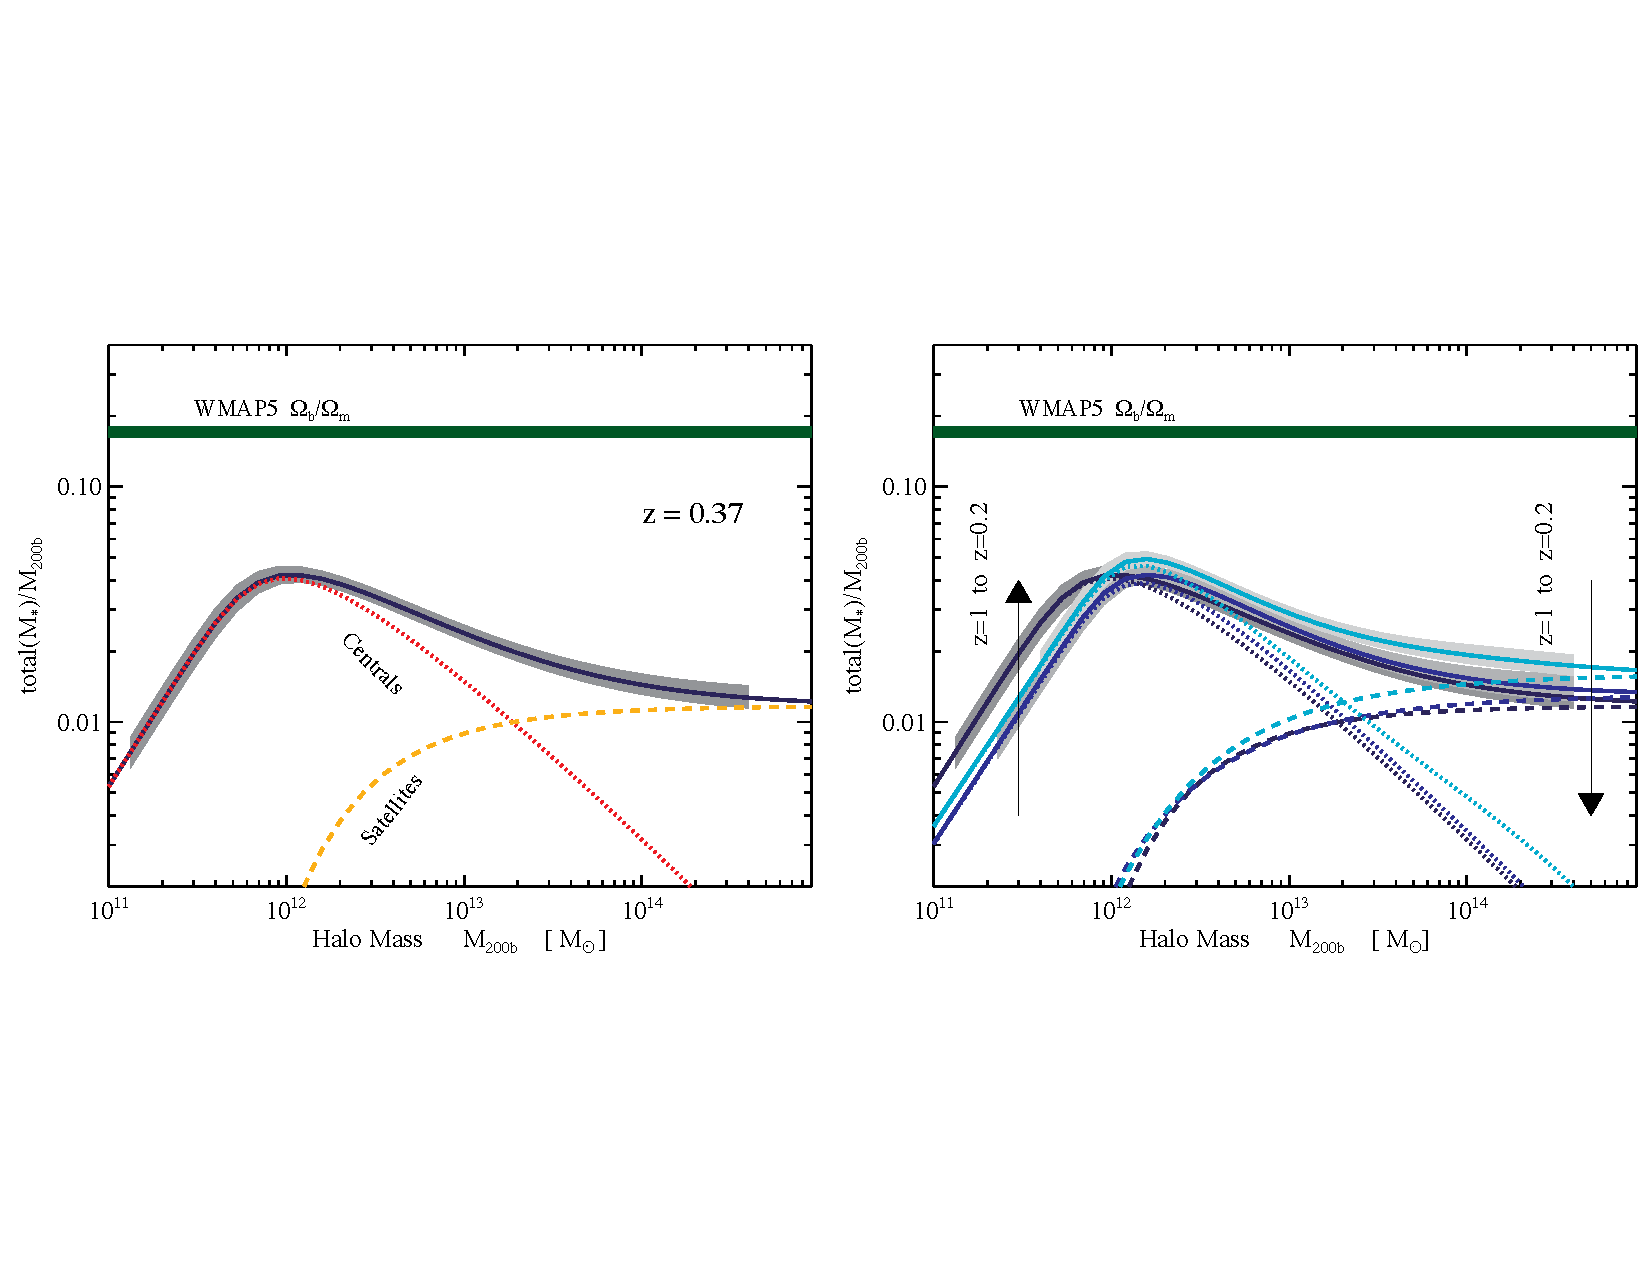
\includegraphics[width=0.9\textwidth]{/Users/palmese/work/PhD_thesis/thesis_format/chapters/chapter1/figs/total_stellar_content_feb18a.pdf}\caption{Total stellar content locked up in galaxies as a function of halo mass compared to the cosmic baryon fraction measured by the Wilkinson Microwave Probe (WMAP5; Dunkley et al. 2009). Left panel: Our prediction from the z1 bin m ($z < 0.37$). Right panel: Our three redshift bins. z1 is shown by the solid dark blue line, z2 is shown by the blue line, and z3 is shown by the turquoise line. Dotted lines show the contribution to Mtot from the central galaxy and dashed lines show the contribution from satellite galaxies. Shaded regions represent the errors on M tot /M . M tot is dominated by the central galaxy at $M < 2 \times 10^{13} M_\odot$ and by satellites at $M_h > 2 \times 10^{13} M_\odot$.}
%\end{figure}

%\section{Galaxy evolution}
%non-DE
%For a review on galaxies physical properties see \citet{blanton09}
%Halo model\\
%LF/SMF\\


%From \citet{lauthaud}:
%The transition between the two regimes is driven by the steep decline in Mcen/M at $M > 10^{12} M_\odot$ . This decline occurs as the contribution from satellites begins to rise. One might then naturally ask if central galaxies in group-scale halos experience stunted growth simply because stellar mass is accumulating within the halo in the form of satellite galaxies, instead of merging onto the central galaxy. Figure 16 reveals that this is not the case. Indeed, the solid line in this Figure demonstrates that the total stellar mass fraction of halos declines at $M > 10^{12} M_\odot$.


%%%%%%%%%%%%%% GW %%%%%%%%%%%%%%%%

\section{Gravitational waves}\label{sec:introgw}

The first detection of gravitational waves (GW) in 2015 (\citealt{ligogw150914}), which was worthy of a Nobel prize in 2017, and of an electromagnetic (EM) counterpart to a GW event (\citealt{MMApaper}) mark the beginning of a new era of astronomy.

Gravitational waves were predicted by Einstein in 1916 (\citealt{einstein1}; \citealt{einstein2}) within the Theory of General Relativity, and scientists had been searching for them for decades before the first detection. GWs are ripples in the space--time that travel at the speed of light,\footnote{At least within GR predictions. We shall see below that the speed of GWs has been confirmed to be the same as the speed of light, or very close to it.} and are a consequence of Einstein's equations. Suppose that there is a small perturbation $h_{\mu\nu}$ on a nearly flat spacetime, i.e. a Minkowski spacetime with a metric $\eta_{\mu\nu}=diag(-1,1,1,1)$. Then the metric will be:
\begin{equation}
g_{\mu\nu}=\eta_{\mu\nu}+h_{\mu\nu}({\bf x}) \quad {\rm with}\, |h_{\mu\nu}| \ll 1\,.
\end{equation}
In this ``linearised gravity'' regime, in the Lorentz gauge (which is equivalent to a coordinate choice), Einstein's equations simplify to (in vacuum, $T_{\mu\nu}=0$):
\begin{equation}
\Big( -\frac{\partial^2}{\partial t^2}+\nabla^2 \Big) h_{\mu\nu}({\bf x})=0\,,
\end{equation}
which is an ordinary wave equation propagating at the speed of light. Plane waves of the type $h_{\mu\nu}=A_{\mu\nu}{\rm exp} (2\pi i k_\mu x^\mu)$ are a solution, with $k_\mu k^{\mu}=0$. If in addition to the Lorentz gauge, one assumes the so called transverse--traceless gauge (which is also allowed because we have 4 degrees of freedom to specify), and chooses the $z$ axis to be along the direction of wave propagation, the line element can be written with 2 only independent amplitudes, $h_+$ and $h_\times$, 2 independent degrees of freedom for the polarization. It can be shown that the metric perturbation becomes (see e.g. the review by \citealt{riles}):
\[
h_{\mu\nu}({\bf x})=
  \left( \begin{array}{cccc}
   0 & 0 & 0 & 0\\
   0 & h_+ & h_\times & 0\\
   0 & h_\times & -h_+ & 0\\
   0 & 0 & 0 & 0\\
  \end{array}  \right) {\rm exp}[ik(z-t)]\, .
\]

\subsection{Detection}
In order to measure these distortions of spacetime, one needs to define some standard ``ruler'' that is not affected by gravity. The speed of light is a quantity which is not affected by the tidal forces: the idea is to send light to a point where it can be reflected, and measure the return time on a clock at the initial position. Given that we want to measure the proper distance between the initial and reflecting point in order to detect any changes in spacetime, we also need to measure the proper time (i.e. in an inertial frame). The return time of the light beam gives us a measurement of that proper distance. In the simple case in which $A_{xy}=h_\times=0$, the wave propagates with a $+$ polarisation along the $z$ axis, and a photon emitted at time $t$ reaches the position $x=L$ at the time:
\begin{equation}
t_L=t+\int_0^L[1+h_+(t(x))]^{1/2} {\rm d} x \,,
\end{equation}
and in the linearised theory the rate of change of the return time $t_{\rm ret}$ of the photon is:
\begin{equation}
\frac{{\rm d}t_{\rm ret}}{{\rm d}t}=1+\frac{1}{2}[h_+(t+2L)-h_+(t)] \,. \label{eq:tret}
\end{equation}
Note that this change depends on the wave amplitude at the origin when the photon is sent out and when it returns. In the general case, the return time will depend on the amplitude at the reflecting end, too.
The technology used in the gravitational wave detectors such as the Laser Interferometry Gravitational-wave Observatory (LIGO; \citealt{aligo}) and Virgo (\citealt{avirgo}) utilise this concept through laser beams in very large interferometers. They are enhanced (i.e. with an extra mirror) Michelson interferometers. The length of the arms of these detectors is much smaller than the typical wavelength $\lambda$ of a gravitational wave, so that Eq. (\ref{eq:tret}) can be expanded in $L/\lambda$. Unfortunately, the GW amplitudes are too small to produce any change in time detectable with the accuracy of current clocks. However, a measurement of such amplitudes can be made by comparing the variation of the return time in perpendicular directions, as in the arms of interferometers.\footnote{This comparison is allowed by the fact that gravitational radiation is not isotropic.} The length of the arms are typically very large ($L=4$ km for LIGO, 3 km for Virgo) to increase the precision on the actual measured quantity, the \emph{strain} $h=\Delta L/L$, where the change in length $\Delta L$ is due to a gravitational wave and is limited by instrumental and environmental noise. A typical amplitude for a gravitational wave generated by a compact binary system merger at the distance of the Virgo cluster is $h\sim 10^{-21}$. For a detector arm of length 4 km, this corresponds to measuring a change in length of 1/1000 the size of a proton. The strain sensitivity of the detectors depends on the frequency of the wave, and it lies between $10^{-20}-10^{-23}$ for the last LIGO-Virgo observation run over the expected range of compact object binaries frequencies. The strain is comparable to the GW amplitude because a detector with arm length $L$ responds to a GW of amplitude $h$ as $\Delta L \sim hL$. The instruments have recently been upgraded to \emph{advanced} LIGO (aLIGO) and Virgo (AdV or aVirgo), with an increased sensitivity of an order of magnitude, corresponding to an increase in search radius of a factor 10, and therefore of $10^3$ in volume. The previous instrument sensitivity was too low for the rate of observable events to detect anything with decent probability.

Given that the wavelength of the GW events is much larger than the detectors' length, they can be thought of as antennas that are only able to localise the position of the GW source over broad areas. Triangulating a detection with multiple interferometers can help in constraining the position: a pair of detectors restricts the location to an annulus over the sky, and combining pairs of detectors at different locations allows intersections of these annuli. LIGO interferometers are located in isolated areas by Washington (LIGO Hanford) and Louisiana (LIGO Livingston), and separated by $\sim 3,000$ km, while Virgo is in Pisa (Italy).

Note that the calculations shown in the linearised gravity are only meant for a qualitative understanding, and more sophisticated calculations need to be performed in a practical analysis. For more detailed analyses of gravitational waves, detectors and searches see the reviews by \citet{Sathyaprakash}, \citet{pitkin} and \citet{riles}.

\begin{figure}\centering
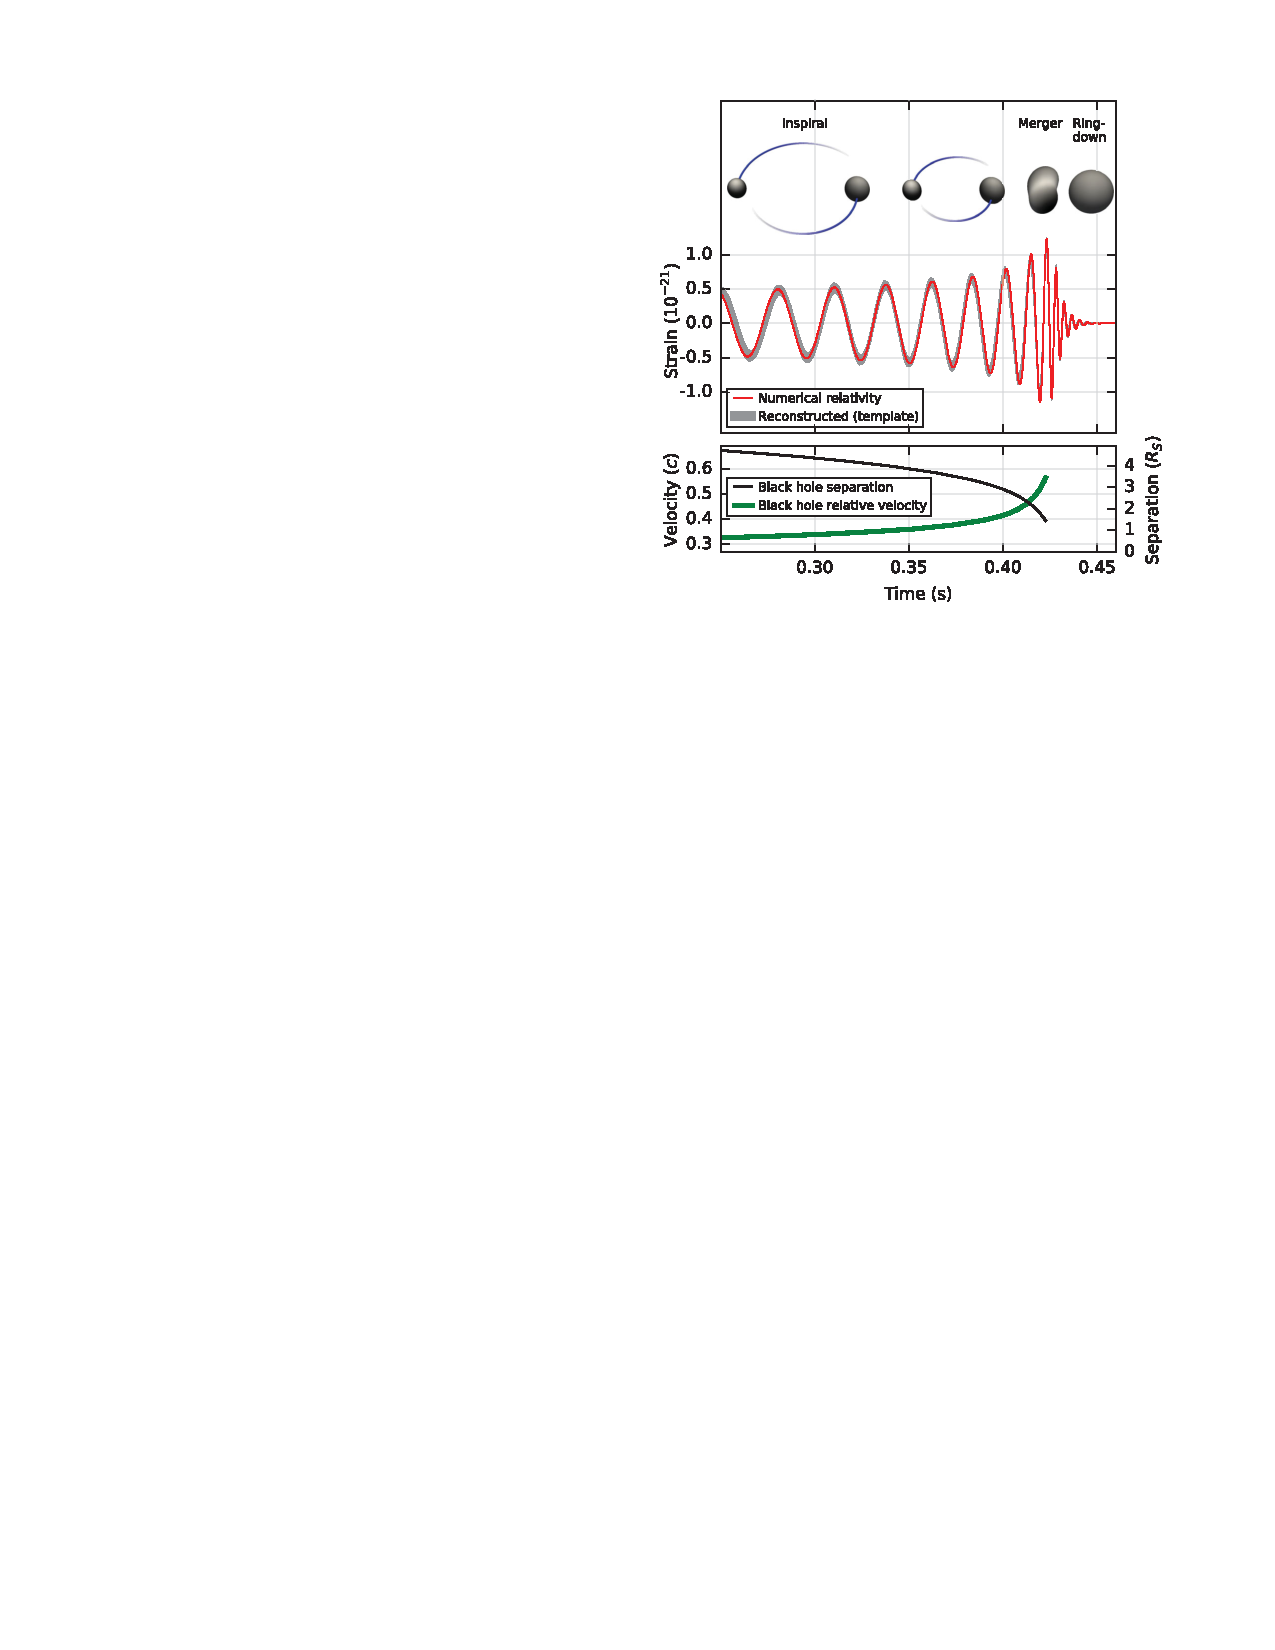
\includegraphics[width=0.7\textwidth]{/Users/palmese/work/PhD_thesis/thesis_format/chapters/chapter1/figs/GWstrain.pdf}
\caption{Strain amplitude from GW150914, showing the different stages of the binary coalescence and the behaviour with time of the oribital velocity and separation. From \citet{ligogw150914}.}\label{fig:strain}
\end{figure}

\subsection{Sources of GWs}
The most promising sources of gravitational waves detectable by current and upcoming GW experiments are mergers of compact binaries (CB). Considered binaries include binary neutron stars (BNS or NS-NS), binary black holes (BBH or BH-BH) and black hole-neutron star (BH-NS) systems. These systems tend to gradually lose angular momentum while radiating gravitational waves, so that their orbit shrinks as they proceed towards an inevitable collision. The gravitational radiation emitted during the highly relativistic final moments of this process is huge, corresponding to $\sim 5-10\%$ of the initial mass of the system, and this is why we regard CBs as the most promising sources to be detected from Earth. The stages that characterise a CB coalescence can be distinguished into: \emph{inspiral}, \emph{merger} and \emph{ringdown}. During the inspiral phase, one can use a quasi--Newtonian approximation and work out analytic expressions. It can be shown that the GW frequency $f$ and amplitude $h$ for a binary system of objects with masses $M_1$ and $M_2$ in a circular orbit are (\citealt{riles}):
\begin{equation}
f=\frac{1}{8\pi} \Bigg[ \frac{5^3}{G^5 \mathcal{M}^5(\tau-t)^3}\Bigg]^{\frac{1}{8}} \,,
\end{equation}
\begin{equation}
h=\frac{1}{r}\Bigg( \frac{5 G^5 \mathcal{M}^5}{\tau-t} \Bigg)^\frac{1}{4}\,,\label{eq:h}
\end{equation}
where $\mathcal{M}\equiv (M_1M_2)^\frac{3}{5}/(M_1+M_2)^\frac{1}{5}$ is the \emph{chirp mass},  $\tau$ is the time at coalescence and $r$ is the distance to the system. Note that: (i) both frequency and amplitude depend on the chirp mass, so we can estimate its value from a GW measurement, but that at this level one cannot disentangle the values of the two masses; (ii) the frequency diverges as $t\rightarrow \tau$; (iii) the amplitude, effectively our observable, declines as $1/r$, which on cosmological scales has the meaning of luminosity distance. An example of strain signal is shown in Figure \ref{fig:strain}. Other parameters are needed to fully describe the binary system, such as orbit ellipticity, object spin and system orientation.

As the radius of the orbit approaches zero, the post--Newtonian approximation breaks down and numerical simulations are required. The coalescence is expected to form a black hole highly distorted in shape. The remnant is expected to go through a ``ringdown'' phase during which these ``distorsions'' are radiated away through GWs.

Other sources of GW signals include continuous waves from spinning neutron stars and primordial GW background, but these topics go beyond the scope of this thesis.

\subsection{The electromagnetic counterpart}

While no electromagnetic emission is expected from the collision of two black holes due to the lack of baryonic material,\footnote{Supermassive black holes (SMBHs) may be an exception, but they are not observable with current and near term GW experiments because of their typical strain and frequency values. Future GW experiments such as LISA may be able to detect SMBH mergers, but we do not consider those in this thesis.} the merger of a compact object system containing a NS should produce a range of different transients emitting at different wavelengths, from radio to gamma-ray, and with different timescales (e.g \citealt{bloom09}; \citealt{EMreview}; \citealt{piran}; \citealt{rosswog}). Let us shortly review the processes that lead to such emission, shown in the schematic cartoon in  Figure \ref{fig:cartoon}, as predicted by popular models and simulations.

\begin{figure}\centering
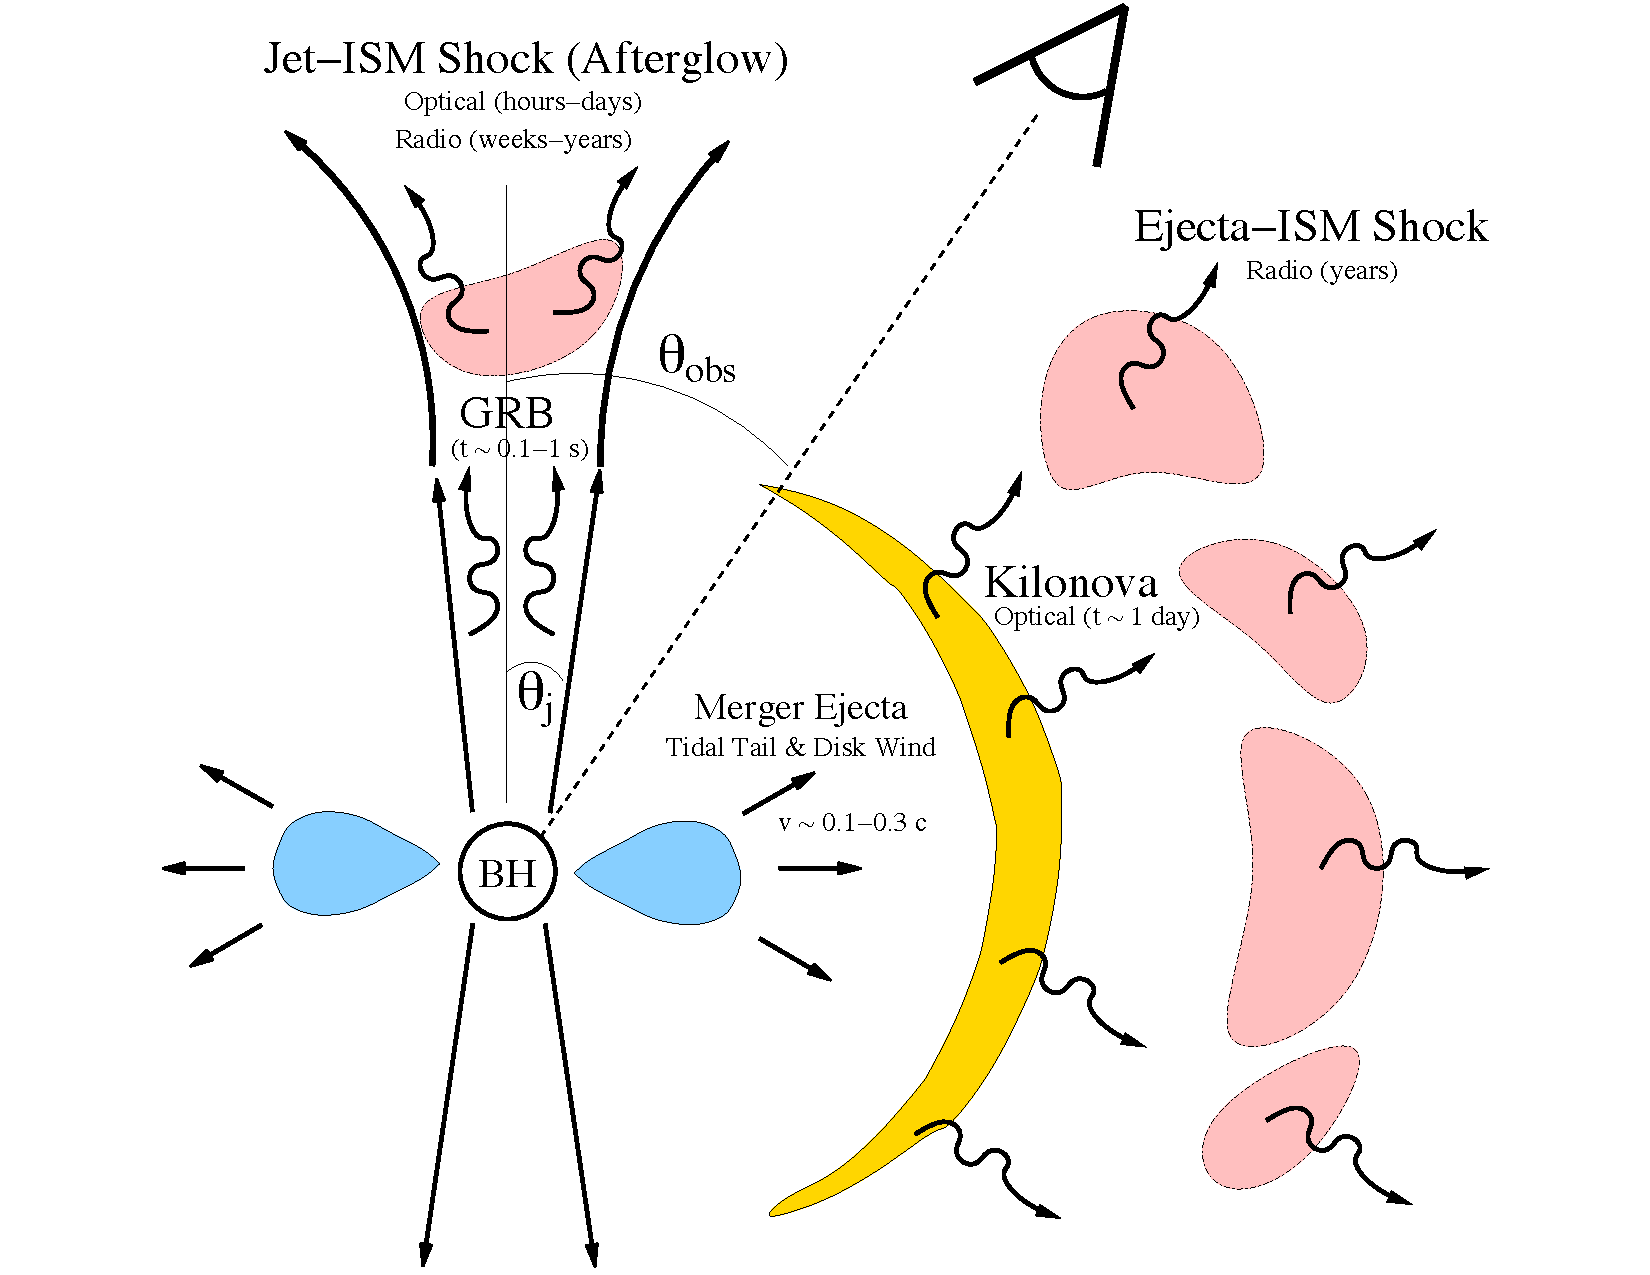
\includegraphics[width=0.6\textwidth]{/Users/palmese/work/PhD_thesis/thesis_format/chapters/chapter1/figs/cartoon.pdf}
\caption{A schematic cartoon of the origin of the predicted EM counterparts to BNS or NS-BH binaries. From \citet{Metzger}.}\label{fig:cartoon}
\end{figure}

First, depending on the final baryonic mass $M_{\rm rem}$ of the binary after the coalescence, the remnant can be a massive, shortly--lived NS, that will eventually collapse into a BH in a matter of milliseconds to seconds. This happens if $M_{\rm rem}\lesssim f M_{\rm max}$, with $f=1.3-1.6$ and $M_{\rm max}$ being the maximum mass of a NS (\citealt{Bauswein}). Otherwise, if the mass of the binary is larger than this limit, the remnant is directly a BH. 

At the time of the merger, part of the binary mass can be ejected in equatorial radial ejecta, part in polar ejecta, where lighter $r$--process\footnote{Rapid--neutron capture processes, or $r$--processes, are a set of nuclear reactions that allows nuclei to capture neutrons more quickly than their radioactive decay. This processes allow the formation of heavy nuclei and occur in regions with high neutron densities (such as NSs).} elements are synthesised. The merger is also expected to produce a centrifugally--supported disk around this remnant. A rapid accretion of the disk is able to power a collimated relativistic jet within seconds from the merger, which can be seen as a short Gamma Ray Burst (sGRB)\footnote{GRBs are classified as short or long, depending on the amount of time during which they are detected (smaller or greater than 2 s).} if observed with a viewing angle $\theta_{\rm obs}\lesssim\theta_j$, where $\theta_j$ is the half--opening angle of the jet. 

A non--thermal GRB afterglow, i.e. the emission that follows the GRB at longer wavelengths, is expected to be produced by the interaction of the jets with the surrounding medium. The afterglow is observed in the optical over timescales up to days or weeks by observers at $\theta_{\rm obs}\lesssim2 \theta_j$. An isotropic radio afterglow is expected to be produced when the jet decelerates to moderate relativistic speeds by shocking the inter--stellar matter (ISM).

Slower expanding disk outflows occur on a timescale of $\lesssim$ seconds post--merger, and constitute another site for $r-$process ejecta. Heavier elements, such as gold and uranium, are produced there. The disk ejecta expand quasi--spherically, and radioactive heating is produced by the radioactive decay of the $r-$process nuclei. This powers the isotropic optical-near infrared emission that lasts over timescales of days to 1 week. This emission is what we call a \emph{kilonova},\footnote{Fun fact: the predicted peak luminosities (\citealt{Metzger+10}) of disk ejecta were $\sim1000$ times those from classical novae.}  and it has been identified by \citet{EMreview} as the most promising EM counterpart, given its isotropic nature, as opposed to the collimated GRB. Kilonovae can show a ``blue''  and fast evolving (over timescales of $\lesssim 1$ day, \citealt{Metzger+10}) component in addition to a ``red'' and longer lived one (\citealt{barneskasen,Tanaka}), depending on the electron fraction of the ejecta, and the elements produced. If ejecta contain lanthanides (atomic numbers $57<Z<71$) or actinides ($89<Z<103$), their optical opacity is higher than what it would be with lighter elements, and this delays the observed evolution of the emission which is also shifted towards redder wavelengths.

An analysis of the expected EM counterparts at different wavelengths is described in \citet{EMreview} and \citet{Metzger17} (in the light of GW170817), while a specific review on kilonovae is presented in \citet{Metzger}. These reviews have been mostly followed when writing this introductory section.

There are several motivations to search for the EM counterpart to a GW event:
\begin{itemize}
\item The closest to a cosmologist's heart is surely the possibility of constraining the Hubble constant. Recall from Eq. (\ref{eq:h}) that we can estimate the luminosity distance from the GW amplitude, and if an EM counterpart is detected and associated with an host galaxy having a measured redshift, then $H_0$ can be constrained through Eq. (\ref{boh}). In other words, GW triggers with an identified EM emission can be used as \emph{standard sirens} (\citealt{Schutz86,Holz05}), similarly to what is usually done with Supernovae as standard candles. This analysis has been performed for GW170817 in \citet{gw170817h0}, and a larger number of GW triggers with an associated EM counterpart will place competitive constraints on $H_0$ (\citealt{Nissanke+10}).
\item To constrain gravity models through estimates of the difference between the speed of light and the speed of gravitational waves (\citealt{Nishizawa16}, \citealt{2017PhRvD..95f3512B} and references therein). In fact, we have seen how GR predicts that GWs propagate at the speed of light. The time elapsed between the detection of the GW signal and the detection of the GRB is at least partially intrinsic to the kilonova model we have described, but it can rule out gravity theories that predict a larger time delay in between the two signal due to their different velocities. This analysis has been performed in \citet{gwspeed}.
\item To study the astrophysics of these systems to constrain the equation of state of NSs and the origin of the $r-$process elements.
\end{itemize}

\subsection{LIGO--Virgo GW triggers}

Coalescences of compact binaries were indeed observed during the first observing runs. 
During the first observing run (O1, September 2015 -- January 2016) only the two LIGO detectors were working, with a sensitivity out to $60-80$ Mpc for BNS. During O1 there were two detections of BBH mergers (GW150914, \citealt{ligogw150914}, and GW151226, \citealt{GW151226}) and a lower significance candidate (LVT151012, \citealt{lvc}).
During O2 (November 2016 -- August 2017) aLIGO was able to detect BNSs out to 100--220 Mpc, and it was joined for the last month by aVirgo, with a horizon reaching 50-60 Mpc (\citealt{ligobns}). Four detections were made during O2: three BBH coalescences (GW170104, \citealt{GW170104}, GW170608, \citealt{GW170608}, and GW170814 \citealt{GW170814}) and a BNS merger (GW170817, \citealt{ligobns}).

\begin{figure}\centering
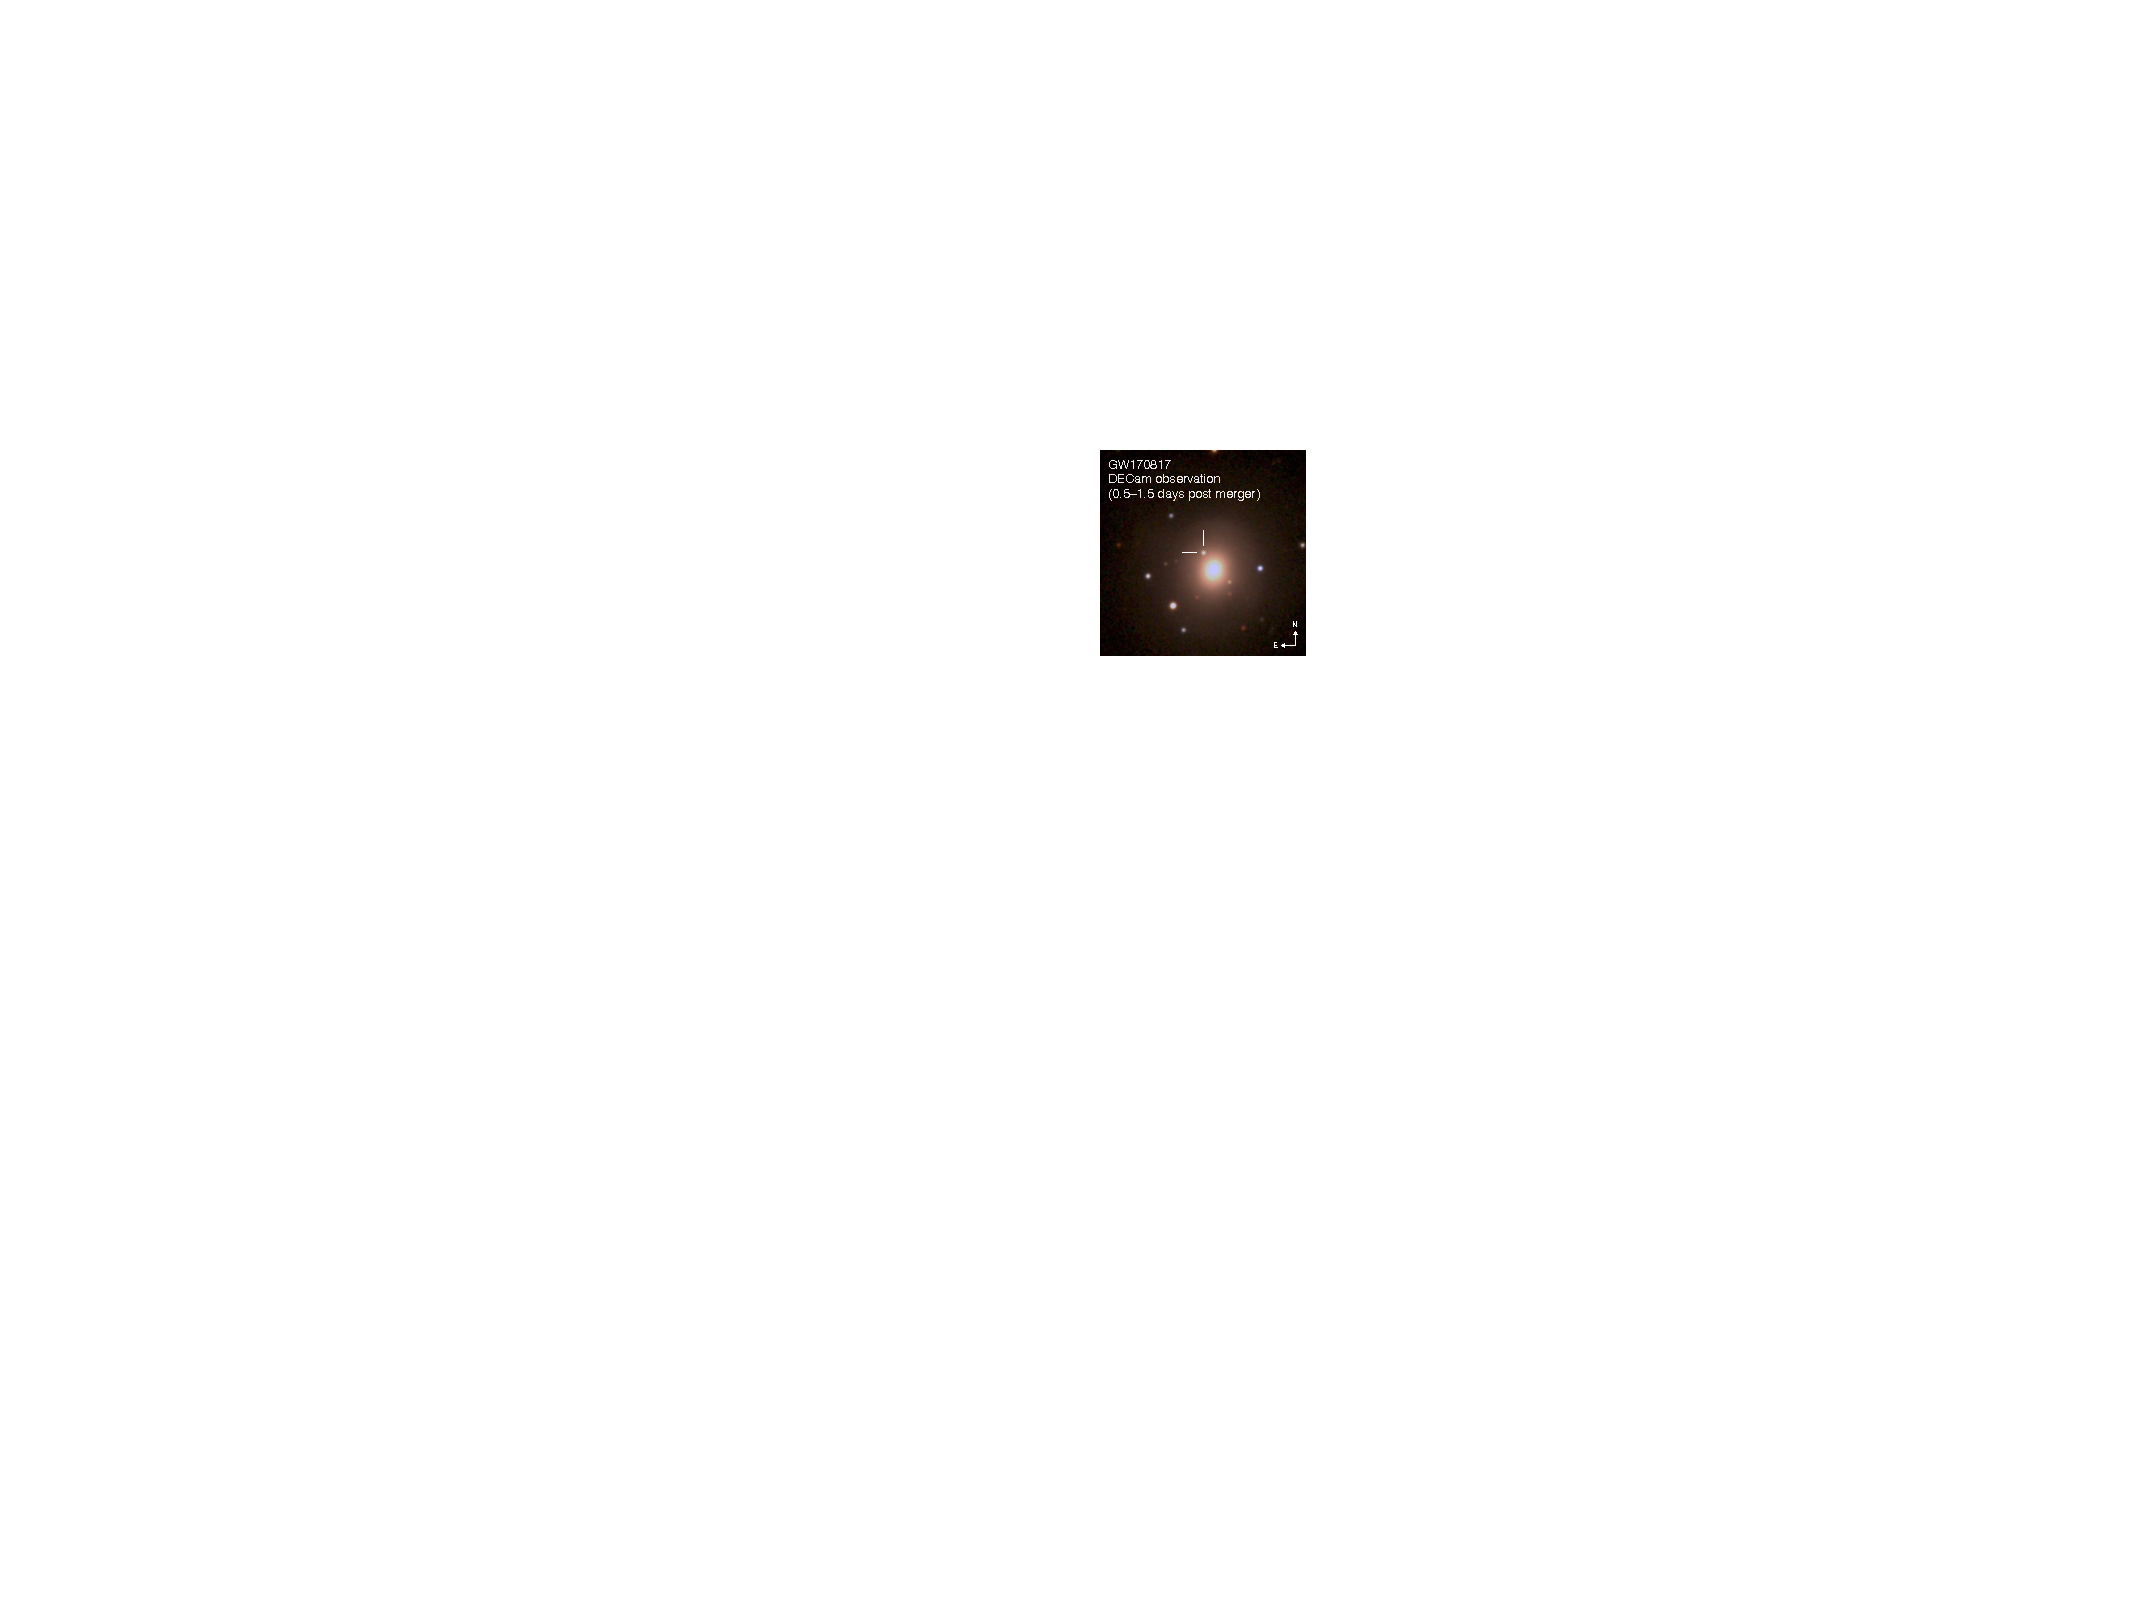
\includegraphics[width=0.5\textwidth]{/Users/palmese/work/PhD_thesis/thesis_format/chapters/chapter1/figs/GW170817_1d.pdf}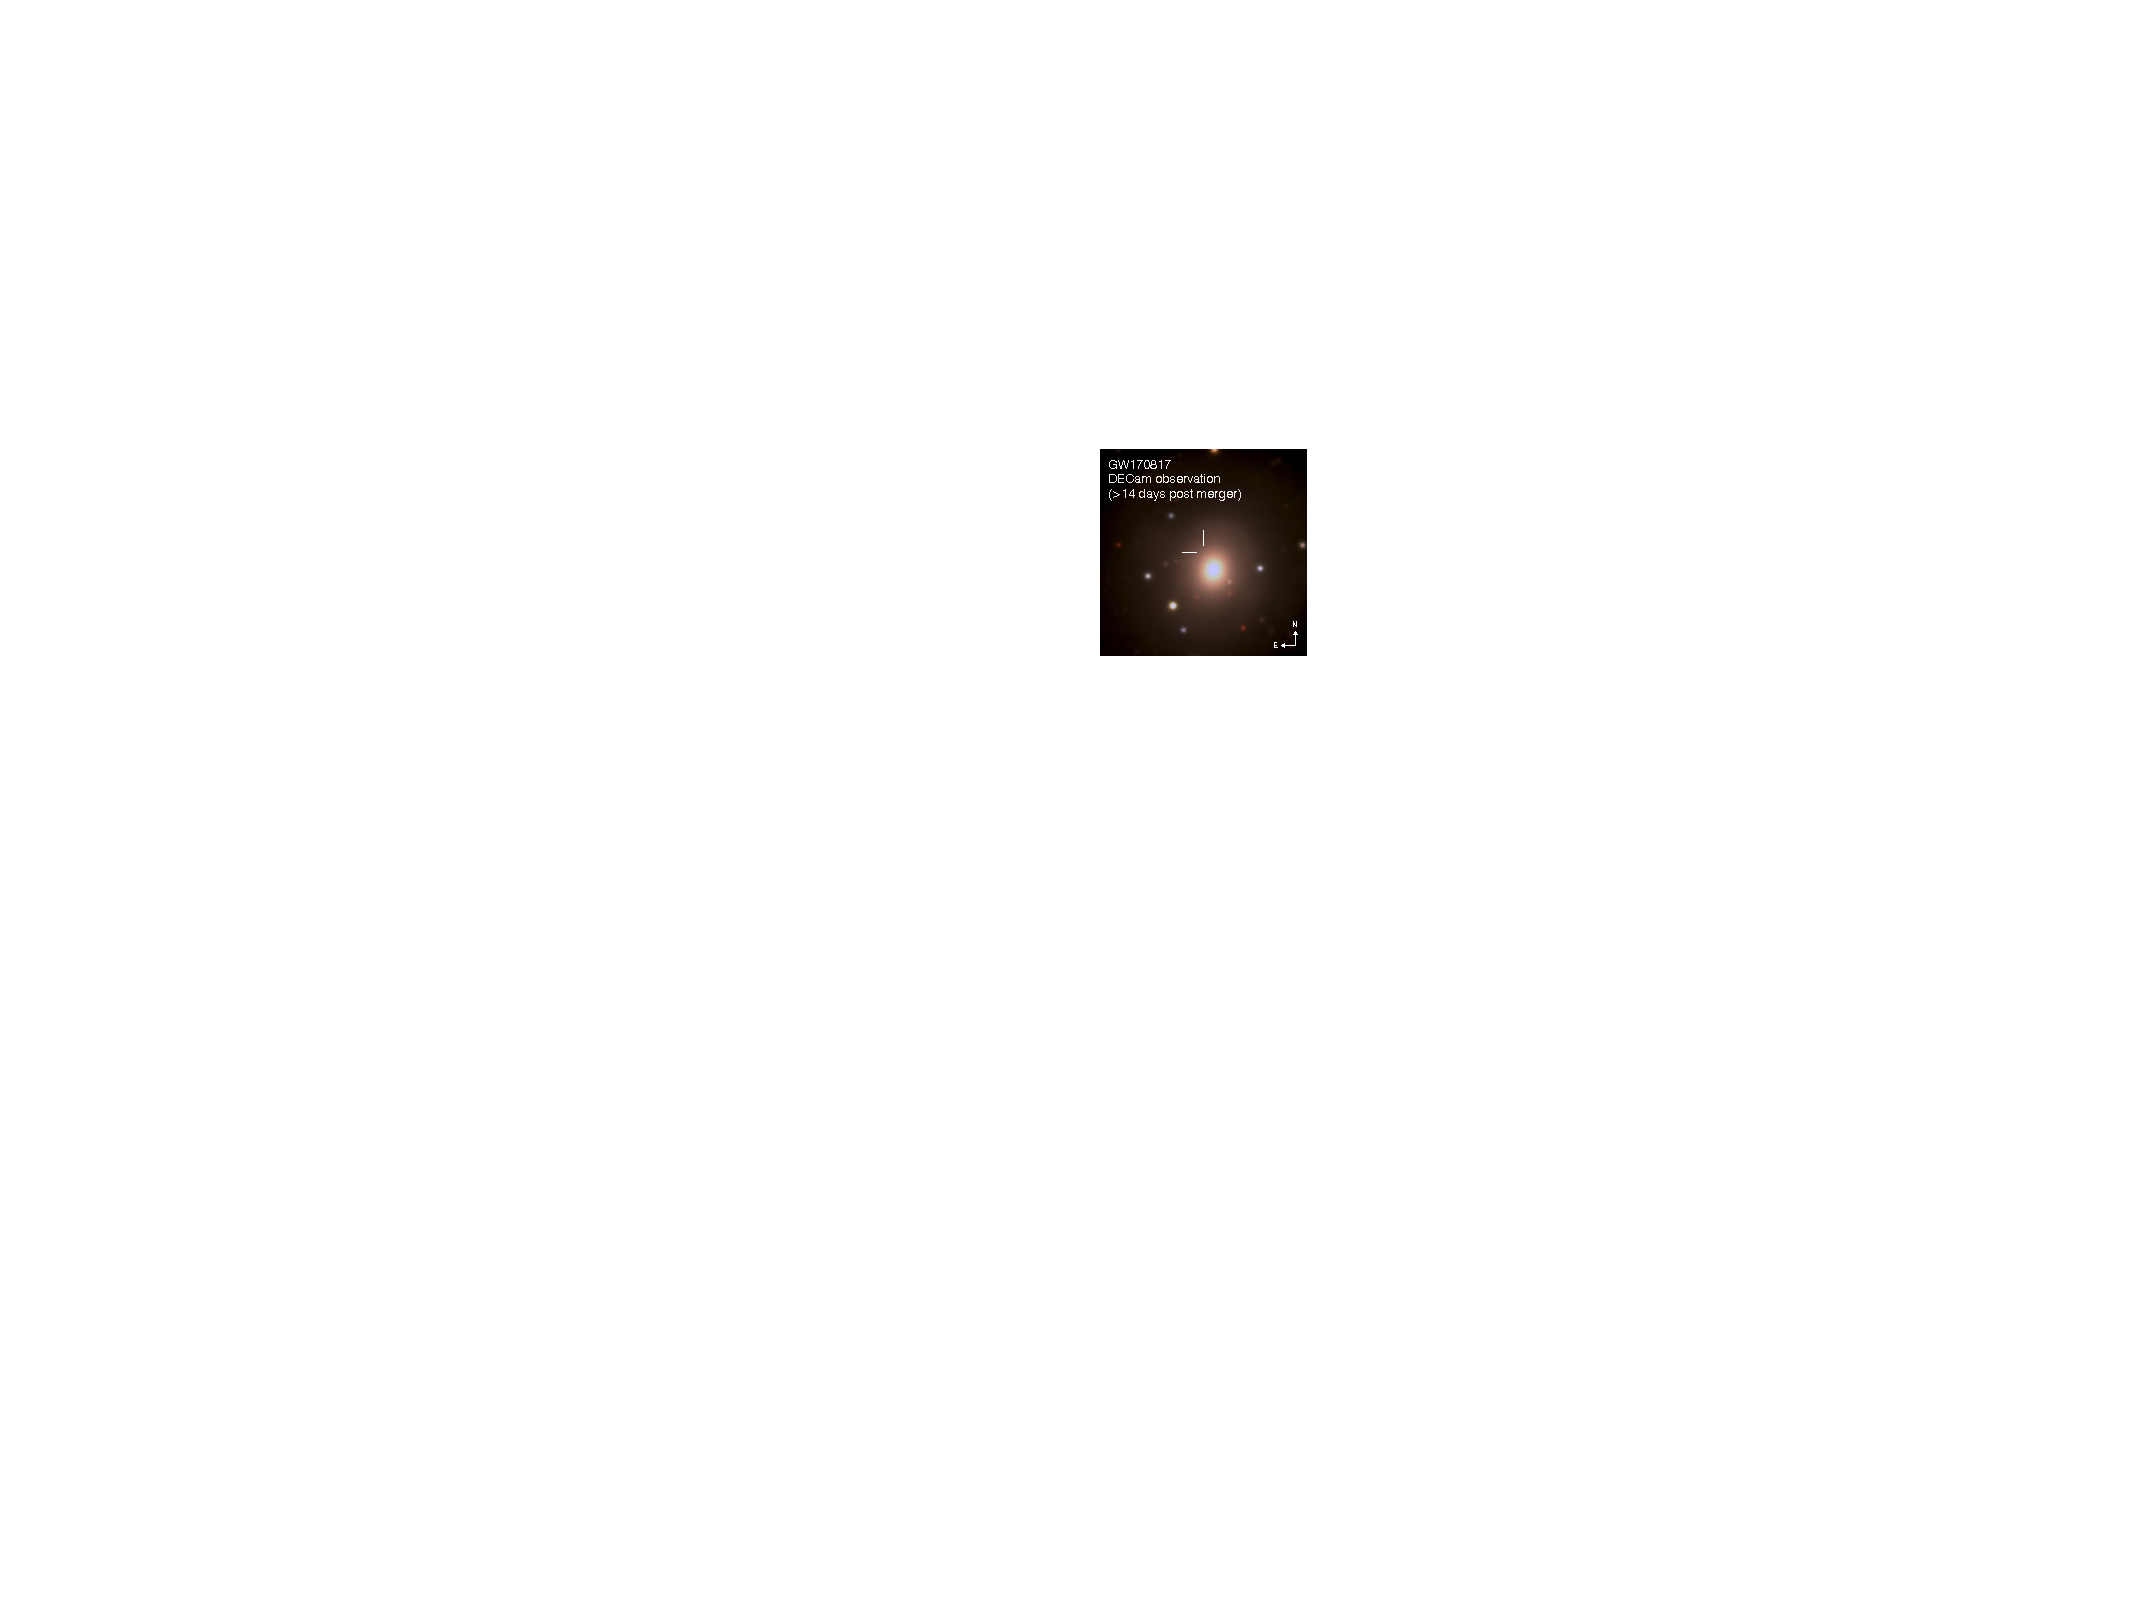
\includegraphics[width=0.5\textwidth]{/Users/palmese/work/PhD_thesis/thesis_format/chapters/chapter1/figs/GW170817_14d.pdf}
\caption{DECam observations of the kilonova  associated to GW170817. Left panel: coadded image from 0.5--1.5 days post GW trigger. Right panel: coadded image after two weeks from the trigger. The transient has significantly faded away within this timescale, as expected from kilonova models. From \citet{marcelle17}, credits to Will Hartley.}\label{fig:bnsDECam}
\end{figure}

GW170814 was the first detection made by LIGO together with Virgo, and the triangulation of the signal permitted a reduction of the $90\%$ sky localization area from 1160 ${\rm deg}^2$ (with LIGO only) to $60~{\rm deg}^2$. All of the mentioned BBH coalescence detections feature black holes of masses $\sim 20-30~M_\odot$, which are not usually expected within standard stellar evolution theories. It is usually thought that BH of stellar origin can hardly reach these masses due to the large mass loss from stellar winds in the late phases of a massive star life. However stellar evolution models of these late stages are uncertain, and \citet{stellarBH} show that BHs of up to $80~M_\odot$ can have a stellar origin. The study of the origin of these black holes has started to involve more exotic models, including Primordial Black Holes (PBH, e.g. \citealt{pbh}), and it provides the opportunity of constraining the amount of dark matter present in the Universe in the form of PBHs (e.g. \citealt{2017JCAP...09..037R}). Typical luminosity distances of these events are 200--400 Mpc.

GW170817 was the first GW event for which an EM counterpart was confirmed (\citealt{MMApaper}). A description of the EM counterpart to this event with DECam data is presented in Chapter 3. In the meantime, we present a DECam coadded image of the first observed kilonova on the left--hand panel of Figure \ref{fig:bnsDECam}.

For a discussion on past and future observing plans with LIGO, see \citet{GWprospects}.

So far, we have discussed how gravitational waves events can have an associated optical counterpart, and how the redshift of the host galaxy is needed in order to make cosmological measurements. We have also discussed how galaxy clusters can constrain cosmology and how they represent an interesting and peculiar environment for galaxy evolution studies. It is now time to introduce the source of data necessary to such analyses: the large galaxy surveys.


%%%%%%%%%%%%% SURVEYS %%%%%%%%%%%%%%%%%%

\section{The era of large galaxy surveys}\label{sec:surveys}

A remarkable number of on--going and planned galaxy surveys will provide data for hundreds of millions, or even billions, of galaxies back to when the Universe was only a fraction of its present age. These surveys were born and funded with the goal of measuring dark energy and other cosmological parameters with unprecedented accuracy.
The constraining power of a particular survey or cosmological probe on DE is often quantified in terms of its \emph{Figure of Merit} (FoM; \citealt{huterer}). The FoM is given by the reciprocal of the area of the $95\%$ confidence limit uncertainty ellipsoid for the DE parameters $w_0,w_a$ defined in Eq. (\ref{wa}). In the Fisher matrix formalism\footnote{The Fisher matrix formalism is often used in astronomy and provides a prescription to estimate errors and covariances for the parameters to be estimated from a future experiment, given the specifics of the experiment.} this corresponds to:
\begin{equation}
{\rm FoM} \propto [\sigma(w_0)\sigma(w_a)]^{-1}\, ,
\end{equation}
where $\sigma(w_0)$ $\sigma(w_a)$ are the uncertainties on the parameters.
This choice was first adopted by the Dark Energy Task Force (DETF; \citealt{detf}) as a metric to compare and classify different surveys and methods. 
The DETF divided dark energy experiments into different Stages. Stage I experiments have provided the data that were known at the time of writing (back in 2009) from observations of Type Ia Supernovae (SN), CMB anisotropies, weak lensing and Baryonic Acoustic Oscillations (BAO). Stage II surveys include DE experiments that were on--going. Stage III comprises on--going medium cost experiments that will improve the FoM by a factor of 3--5 compared to Stage II. Stage IV includes large scale, longer term projects that will improve the FoM by a factor of $\sim 10$ compared to Stage II.

\begin{sidewaystable}
 \centering 
 \begin{tabular}{ccccccc}
  \hline
  \hline
  Project&Dates&Area [deg$^2$]&Data & Spec-$z$ range & Probes &Stage \\
  \hline
BOSS & 2008-2014 &10,000 & Opt-S & $0.3-0.7$ (gals) &BAO & III\\
DES & 2013-2019 &5,000 & Opt-I & -- &BAO, WL & III\\
&&&&&CL, SN &\\ 
eBOSS & 2014-2020 &7,500 & Opt-S & $0.6-2.0$ (gal/QSO) &BAO& III\\
SuMIRe & 2014-2024 &1,500 & Opt-I & -- &WL, CL & III\\
&&& Opt/NIR-S & $0.8-2.4$ (gals) &BAO&\\
HETDEX & 2014-2019 &300 & Opt-S & $1.9-3.5$ (gals) &BAO& III\\
DESI & 2019-2024 &14,000 & Opt-S & $0-1.7$ (gals) &BAO& IV\\
LSST & 2020-2030 &20,000 & Opt-I & -- &BAO, WL& IV\\
&&&&& CL, SN&\\
\emph{Euclid} & 2020-2026 &15,000 & Opt-I & -- &WL, CL& IV\\
&&&NIR-S& $0.7-2.2$ (gals) &BAO&\\
\emph{WFIRST} & 2024-2030 &2,200 & Opt-S & -- &WL, CL, SN& IV\\
&&&NIR-S& $1.0-3.0$ (gals) &BAO&\\

\hline
 \end{tabular}
\caption{A selection of major recent, on--going and future dark energy experiments. Abbreviations in the ``Data'' column refer to optical (Opt) or near-infrared (NIR) imaging (I) or spectroscopy (S). For spectroscopic experiments, the ``Spec-$z$'' column lists the primary redshift range for galaxies (gals), quasars (QSOs). %, or the Lyman-$\alpha$ forest (Ly$\alpha$F). 
Abbreviations in the ``Methods'' column are weak lensing (WL), clusters (CL), supernovae (SN) and baryon acoustic oscillations (BAO). %, and redshift-space distortions (RSD). 
Adapted from \citet{weinbergrev}.}\label{tab:surveys}
\end{sidewaystable}

Table \ref{tab:surveys} presents a representative, albeit not exhaustive, list of on--going and upcoming galaxy surveys, both imaging and spectroscopic. Spectroscopic datasets are usually smaller than photometric ones, due to the time involved in taking spectra, and they usually go down to brighter flux limits than imaging surveys. On the other hand, spectra trace in greater detail the fingerprints of galaxies' stellar populations, and can provide better measurements of the stellar chemical composition, redshift, dust content, amongst other properties. As a result, spectroscopic surveys can provide complementary means to constrain galaxy evolution models and cosmology, as well as calibration sets for photometric surveys.

Stage II projects include the famous optical imaging surveys Sloan Digital Sky Survey II (\citealt{sdssII}) and PanSTARRS I (\citealt{panstarss1}), and the \emph{XMM} Cluster Survey (\citealt{romer}) in the X--ray. Stage III imaging experiments comprise DES, described in Section \ref{sec:DES}, and the Hyper--Suprime Camera (HSC; \citealt{hsc}), carrying out similar observations to DES, but to a greater depth on a smaller area. The HSC is only one part of the greater Subaru Measurement of Images and Redshifts (SuMIRe) project. On the spectroscopic side, the Baryon Oscillation Spectroscopic Survey (BOSS; \citealt{boss}) and it successor extended BOSS (eBOSS; \citealt{eboss}) probe the distribution of millions of galaxies and quasars, and the Hobby-Eberly Telescope Dark Energy Experiment (HETDEX; \citealt{hetdex}) maps a smaller area but out to a greater distance. Stage IV projects feature the optical imaging Large Synoptic Survey Telescope (LSST; \citealt{lsst}), the great successor of DES. LSST will image the southern sky every four nights, providing a huge amount of data for transients science (in particular, SN cosmology). The images will be coadded over ten years of observations, resulting in an incredibly deep survey for a ground based experiment.

Space missions include \emph{Euclid} (\citealt{euclid}) and \emph{WFIRST} (Wide Field Infrared Survey Telescope; \citealt{wfirst}), and will provide both imaging and spectroscopic data for billions of galaxies.

Surely datasets mapping huge volumes of the Universe can be exploited for astrophysical studies beyond cosmological parameters. It is in this spirit that gravitational wave follow up programs were born with the goal of observing kilonovae, and that we perform galaxy evolution studies by looking at the astrophysical properties of single galaxies. In addition, galaxy surveys have enabled observations of the host galaxy to the first BNS GW signal, so that we could provide a measurement of the cosmological parameter $H_0$. In this thesis we also show how galaxy properties can be used to estimate the total mass of galaxy clusters, which again is a necessary step towards cosmological measurements.


\subsection{The Dark Energy Survey}\label{sec:DES}

The DES (for further information see \citealt{descollaboration} and \url{www.darkenergysurvey.org}) is an optical-near-infrared survey that is imaging 5000 ${\rm deg}^2$ of the South Galactic Cap in $grizY$ bands over 525 nights spanning almost six years. The DES filters transmission curves are shown in Figure \ref{fig:filters}. The survey is being carried out using a $\sim3$ $\textrm{deg}^2$ CCD
camera (the DECam, see \citealt{flaugher}) mounted on the Blanco 4-m telescope at the Cerro Tololo Inter-American Observatory (CTIO) in Chile. DES started in 2012 with a testing period (November 2012 -- February 2013) called Science Verification (SV)\footnote{For public data release see: \url{http://des.ncsa.illinois.edu/releases/sva1}}. The data used in this thesis come from SV and from the first three years (Y3) of observations (September 2013 -- February 2016), which cover $\sim5,000~ {\rm deg}^2$ with up to 4 passes per filter. The DES Y3 footprint, which corresponds to the final footprint, is shown in black in Figure \ref{fig:footprint}. Some of the data used (the wide-field coadd source catalogs) is now publicly available at \url{https://des.ncsa.illinois.edu/releases/dr1} and described in \citet{dr1}. Target of opportunity data from the fourth year of observations are also used in the GW follow up work. At the time of writing, five observing seasons have been completed.

\begin{figure}\centering
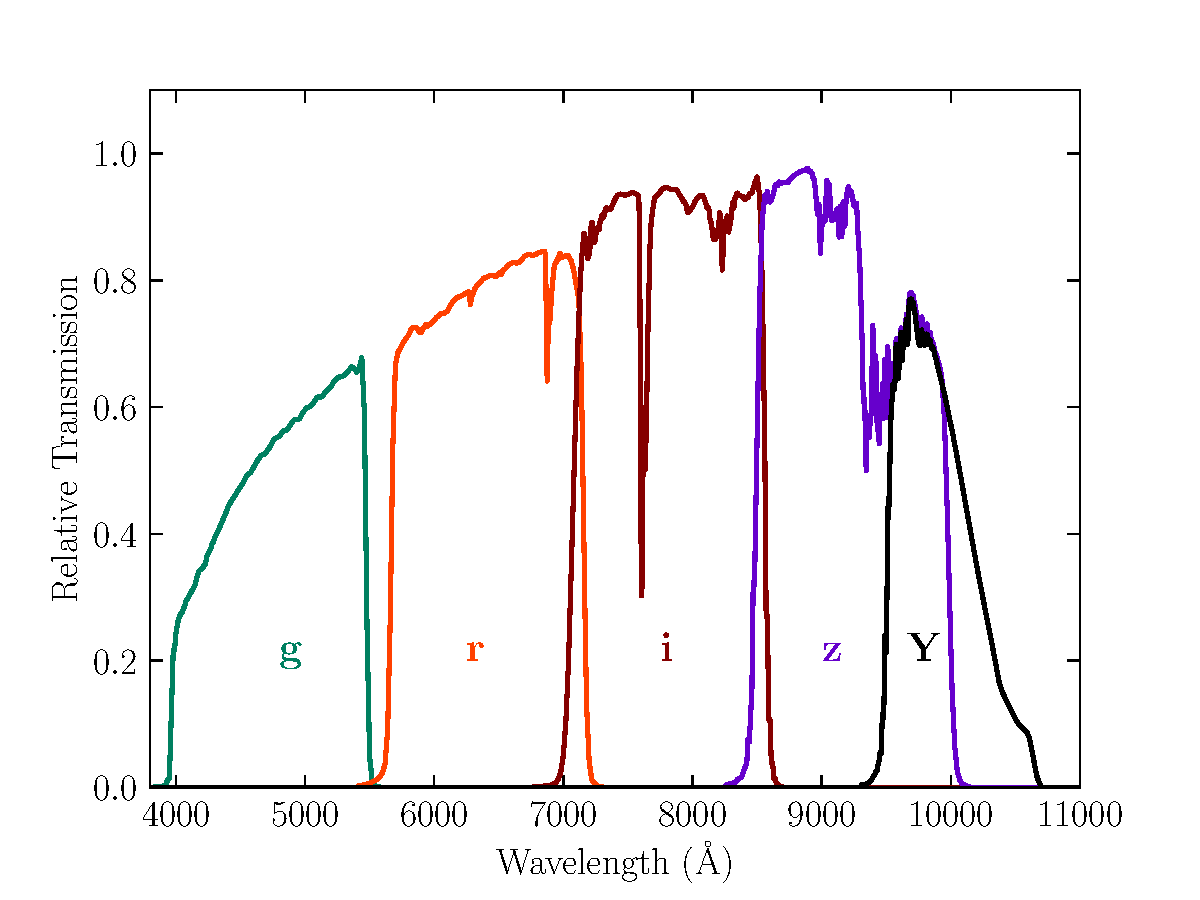
\includegraphics[width=0.6\textwidth]{/Users/palmese/work/PhD_thesis/thesis_format/chapters/chapter1/figs/dr1_bandpass.pdf}
\caption{DES filters transmission curves. From \citet{dr1}.}\label{fig:filters}
\end{figure}
\begin{figure}\centering
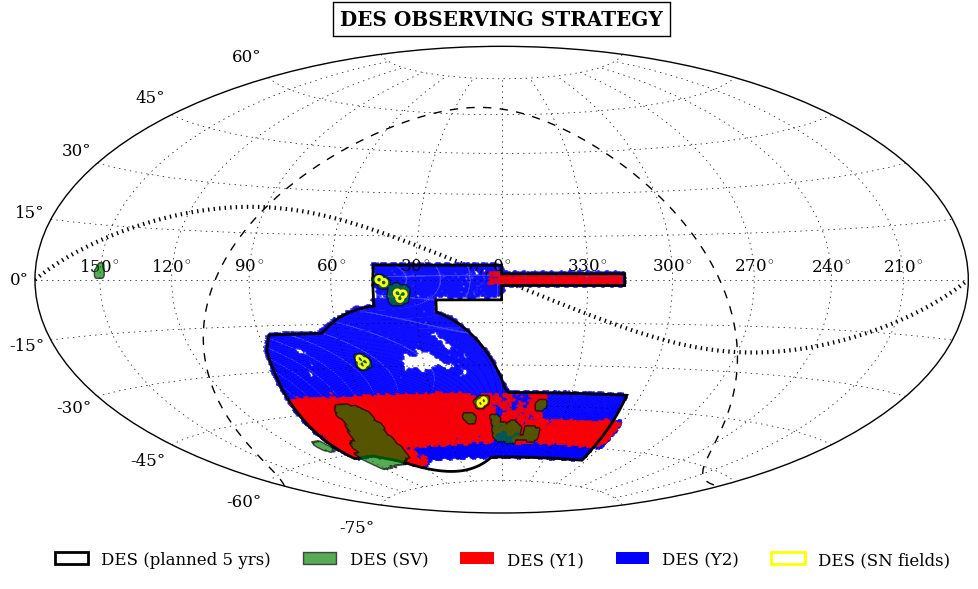
\includegraphics[width=0.8\textwidth]{/Users/palmese/work/PhD_thesis/thesis_format/chapters/chapter1/figs/footprint_Y1.png}
\caption{DES footprint. The green area is covered by the Science Verification data, used in Chapter 2 and 4. The red area represents the observations from the first year of observations, and it is the area studied with the Y1 redMaPPer clusters in this thesis (Chapter 6). The 5 years planned footprint is shown by the black contours, and it is the same area covered by the Y3 data used in Chapters 3, 5 and 6. The difference between Y3 and Y5 is in the number of passes, and therefore the depth. Plot from \citet{nonDE}.}\label{fig:footprint}
\end{figure}

The survey strategy is designed to optimize the photometric calibration by tiling each region of the survey with several overlapping pointings in each band. This provides uniformity of coverage and control of systematic photometric errors. This strategy will allow DES to determine photometric redshifts of $\sim 300$ million galaxies to an accuracy of $\sigma(z) \simeq 0.07 $ out to redshifts above 1, with some dependence on redshift and galaxy type, and cluster photometric redshifts to $\sigma(z) \sim 0.02$ or better out to $z \simeq 1.3$ (\citealt{descollaboration}). It will find $\sim 380,000$ groups and clusters and also provide shapes for approximately 200 million galaxies for weak lensing studies. The final depth of the survey will be similar to that of the SV data, where the median $10\sigma$ depths are $g\sim24.45, r\sim24.30,i\sim23.50,z\sim22.90, Y\sim21.70$. The Supernova fields (shown in yellow in Figure \ref{fig:footprint}) are observed to a greater depth. Observations will be completed in January 2019, while the data processing to release the Y5 galaxy catalogs can take one or two years.

The DES Data Management (DESDM) pipeline was used for data reduction, as described in detail in \citet{sevilla}, \citet{desai} and \citet{dataproc}. The process includes calibration of the single-epoch images, which are co--added after background subtraction and then cut into tiles. The source catalogue was created using \textsc{Source Extractor (SExtractor}, \citealt{sextractor}) to detect objects on the $riz$ co-added images. 

The data from DES will allow high precision measurements of dark energy and dark matter through the four cosmological probes previously described: weak gravitational lensing, galaxy clusters abundance, galaxy angular clustering and Supernovae. Several papers using these methods have recently been published for the early DES data covering the Y1 area, in particular from weak lensing and galaxy clustering (\citealt{Y1key}; \citealt{gruencosmo}; \citealt{DESBAO}; \citealt{DESH0}). The DES collaboration has also been able to publish significant work beyond cosmology and Dark Energy, including Milky Way studies, Trans-Neptunian Objects and much of the work included in this thesis regarding galaxy evolution and gravitational waves. See \citet{nonDE} for an overview on non-Dark Energy studies with DES.\\

The data used in this thesis also includes Anglo-Australian Telescope (AAT) target of opportunity time data. Other publicly available datasets have been used (VHS, HST, 2dF, 6dF, 2MASS).

\section{Thesis Outline and notation}

This thesis is structured as follows:

\begin{itemize}
\item In {\bf Chapter 2} I describe the methods used to derive galaxy properties (mainly stellar mass) and redshifts from galaxies' Spectral Energy Distribution. In particular, I introduce a method that uses a Bayesian Model Averaging technique.
\item In {\bf Chapter 3} I show how large galaxy samples with available redshifts and properties are fundamental for electromagnetic follow ups of gravitational wave events. Furthermore, they can be used to understand the formation and evolution of the binary systems they contain. An analysis of this type is presented for the golden event GW170817.
\item {\bf Chapter 4} includes a study on early DES data showing that stellar masses can be estimated in a robust manner with DES, in particular concerning galaxy clusters. A first estimate of stellar mass fraction in clusters from DES is presented.
\item In {\bf Chapter 5} I introduce a promising cluster mass proxy, $\mu_\star$, based on stellar masses. Its performance is calibrated against X-ray and weak lensing measurements.
\item {\bf Chapter 6} shows cluster evolution results for $\sim 80,000$ DES clusters. We measure the stellar--to--halo mass relation and the stellar mass function for central galaxies and satellites. Other results on central galaxies and ICL are shown.
\item Finally, {\bf Chapter 7} is dedicated to the conclusions of this work and to future prospects for expanding my GW host analyses to binary black hole events and to BNS triggers from the fast approaching third LIGO observing season. The plan for producing $\mu_\star$ for Voronoi--Tesselation clusters over the DES Year 3 area is also already undergoing.

\end{itemize}
Throughout this work we assume a $\Lambda$CDM flat cosmology with $h=0.7$, $\Omega_m = 0.3$, $\Omega_\Lambda =0.7$ unless otherwise stated. The notation adopted for the cluster mass and radius follows the one often used in literature. The radii of spheres around the cluster centre are written as $r_{\Delta m}$ and $r_{\Delta c}$ where $\Delta$ is the overdensity of the sphere with respect to the mean matter density (subscript $m$) or the critical density (subscript $c$) at the cluster redshift. Masses inside those spheres are therefore $M_{\Delta m}=\Delta \frac{4 \pi }{3}r^3_{\Delta m}\rho_m$ and similarly for $M_{\Delta c}$.  In the following, we quote $\Delta=200$, which roughly corresponds to the density contrast at virialisation for a dark matter halo at $z=0$. In order to convert between the different mass definitions we use the Python Colossus tools (\citealt{colossus}). The galaxies' Initial Mass Function adopted follows \citet{chabrier}, unless otherwise stated. Logarithms indicated as Log have base 10.

Errors quoted are $1\sigma$, unless otherwise stated.






